\section{Introduction}
Acquisition of DWB datasets in S\&S mode with overlapping bed positions result in complex datasets of PET RAW data, in relation to timing and positional information. Moreover, the addition of an initial DSB acquisition, commonly conducted for IDIF derivation purposes and providing information that allow for more complex kinetic modeling of the sampled region~\cite{Zaker2020}, increase the complexity of the PET RAW dataset. 

Suggested practices~\cite{Karakatsanis2013} and state of the art implementations~\cite{Hu2020} of DWB protocols regard the two datasets (DSB and DWB) as independent and suggest to perform independent reconstructions on each dataset. Post-reconstruction kinetic model fitting is then used to combine the TAC information over both datasets. 
Furthermore, the DWB dataset contains locations at the overlapping bed regions which are sampled twice as much as central bed regions, as a result of the overlapping sampling necessary to increase sensitivity at the bed position edges. The overlap timing information combines the timing of the adjacent bed positions. In post-reconstruction kinetic modeling, which is applied independently on each voxel TAC, suggested practices make use of modified timing information (average of two bed position timings) for voxels that fall at overlapping regions~\cite{Karakatsanis2013} which result to a degree of degradation of the timing information. Another suggestion is to make use of independent dynamic reconstruction of each bed position from the DWB dataset and apply post-reconstruction overlapping of parametric images ~\cite{Karakatsanis2016a}.
It is important to note that DWB acquired in CBM mode, although free of the need of overlapping bed positions still require similar considerations to be taken into account for each axial location of the DWB acquisition~\cite{Karakatsanis2016b,Hu2020}.

The flexibility offered by the CASToR reconstruction platform that allows for direct reconstruction of multi-bed data~\cite{Ross2004} can be expanded to direct multi-bed dynamic reconstruction with DWB data, using the exact timing information of the dataset and all bed positions within the same iterative loop. Furthermore, the offered flexibility can allow for the use of both DSB and DWB datasets within one unique reconstruction loop.
In this chapter we describe how this novel DWB protocol reconstruction concept was implemented in CASToR and present results from dynamic reconstruction of real DWB data from the IsotoPK study, which were also presented in the EANM2020 conference~\cite{chalampalakis2020EANM}.
Finally we discuss the complications arising from kinetic model fitting errors in dynamic reconstruction with respect to data from DWB acquisitions and present our work towards reduction of these errors using adaptive residual modelling for dynamic reconstruction, as presented in the IEEE-MIC2020 conference. To our knowledge is the first a method of this type has been applied on real DWB data.

\section{Methods}
\subsection{Dynamic Whole Body Datasets}
A diagram of axial position and time for an example three bed position DWB protocol is shown in figure~\ref{fig_3_3:OverlapFraming}, to demonstrate the differences in temporal sampling between central locations and locations at the bed overlapping regions. The bed locations in this example are identical to the setup used for the NHP acquisition on the Signa PET/MR described in chapter~\ref{Chap3_1:AcquisitionOptimization}.
As it can be seen at the left diagram of figure~\ref{fig_3_3:OverlapFraming} axial positions that fall outside of the overlap region result in framing that is equal to the framing of their respective bed positions. Positions over the overlap regions, seen at the right diagram of figure~\ref{fig_3_3:OverlapFraming}, result in framing equal to that of both adjacent bed positions, which gives twice the number of frames compared to locations outside the overlap. Locations at the overlap regions are not sampled continuously from both contributing bed positions due to the interruption by the movement of the bed and system delays.  
Finally, complexity is increased when the DSB data are included, as shown in figure~\ref{fig_3_3:CompleteProtocolFraming}, with that information contributing to different locations of the DWB acquisition that might fall in overlap regions or not depending on the protocol setup. 

\begin{figure} [h!]
\centering
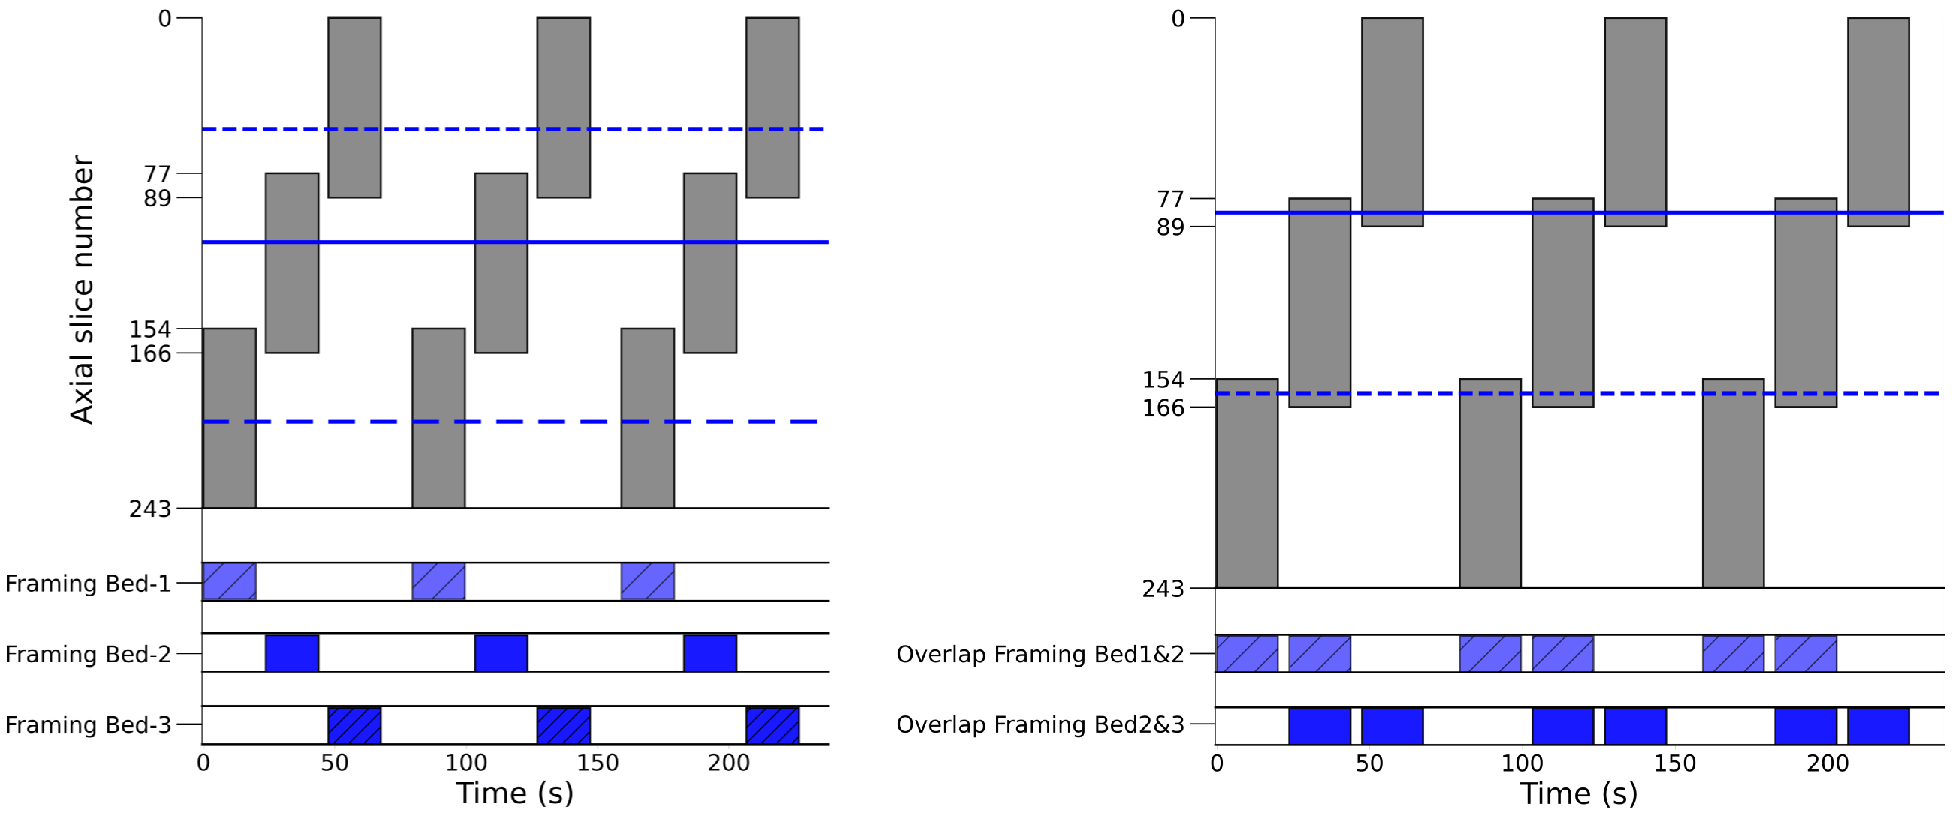
\includegraphics[scale=0.50,angle=0]{3_Results/3_3_DWB_Reconstruction/figures/OverlapTiming.pdf}
\caption{Axial slice number vs time for an example three bed positions DWB acquisition. Central axial slices (left) and slices at the overlapping regions (right) considered for the result framing.} 
\label{fig_3_3:OverlapFraming}
\end{figure} 

\begin{figure} [h!]
\centering
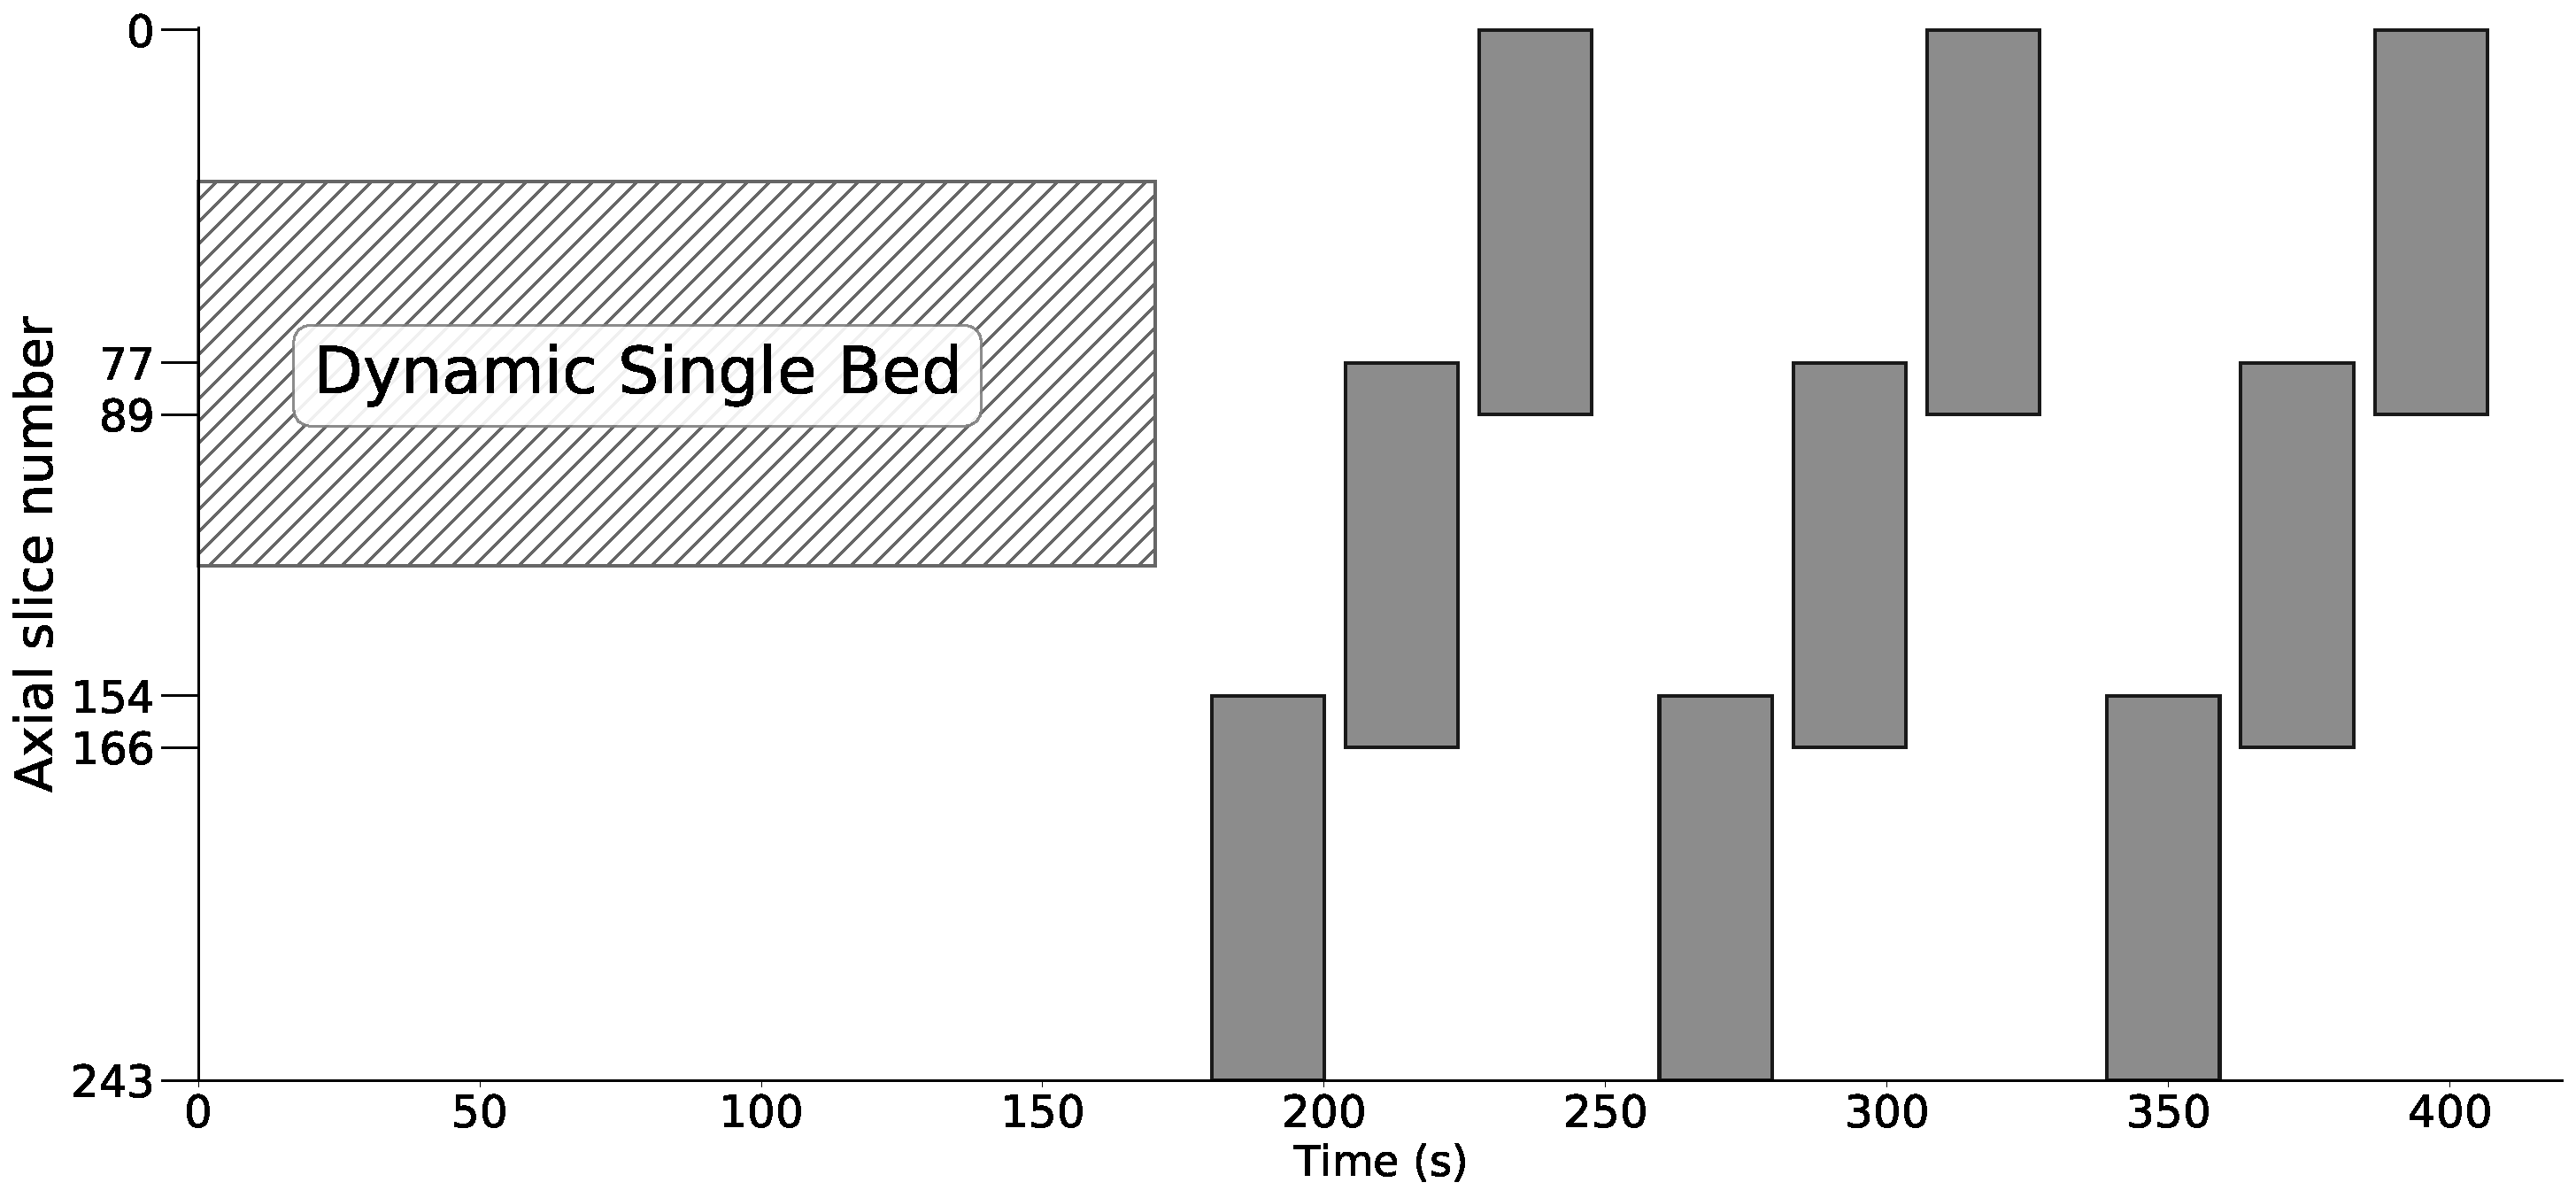
\includegraphics[scale=0.28,angle=0]{3_Results/3_3_DWB_Reconstruction/figures/CompleteProtocolTiming.pdf}
\caption{Axial slice number vs time for an example three bed positions DWB acquisition, including an initial DSB phase of 180 s.}
\label{fig_3_3:CompleteProtocolFraming}
\end{figure} 

If considering only the DWB dataset, with each individual S\&S acquisition as an independent frame, the total number of frames in the DWB dataset will be defined by all the individual S\&S steps.% In the example presented in figure~\ref{fig_3_3:OverlapFraming} the DWB data provide nine frames. 
But not all frames need to be considered for all regions of the effective FOV. 
The choice of the appropriate framing for each location, whether within or outside the overlap, can be made using an mask image that indicates which locations are sampled on each frame. This type of mask could be used for example with post-reconstruction parametric imaging, applied at each voxel to mark which frames need to be considered.

With CASToR the use of multi-bed data can be made directly within a single iterative loop, using the methodology described in section~\ref{chap2_4:MultiBedRecon}. The same framework can be extended to direct multi-bed dynamic reconstruction of DWB datasets, using the same iterative loop. 
For linear dynamic models, dynamic reconstruction (without use of nested optimization) can be applied directly next to the system matrix, as shown in equation~\ref{eqn:4DMLEM}, within a single iterative loop over all dynamic data $y_{ti}$. 

For DWB data, incorporation of the bed offset information in the projection operation can naturally lead to direct multi-bed dynamic reconstruction, where the selection of the sampled time points for the location of a voxel $j$ is conducted by the projection operation. In this case the projection operation and consequently the system matrix elements will depend on the frame $t$. 
This can also be expressed as an extension of the direct multi-bed reconstruction, described by equation~\ref{eqn2_4:MLEM_multibed}, to dynamic reconstruction where the axial offset of each bed position is incorporated in the time dependent information of the system matrix.
This provides
%
\begin{equation}
\theta_{pj}^{(k+1)} = \frac{\theta_{pj}^{(k)}}
{\sum_{t=1}^{n_t} B_{tp} \sum_{i=1}^{n_i} P_{tij}} 
\sum_{t=1}^{n_t} B_{tp}  \sum_{i=1}^{n_i} P_{tij} 
\frac{y_{ti}}
{\sum_{d=1}^{n_j} P_{tid} \sum_{p=1}^{n_p} B_{tp}\theta_{pj}^{(k)} + C_{ti} } \\, \\
\label{eqn:4DMLEM_Multibed}
\end{equation} 

where the set of basis functions $B$ is precomputed for all time frames of the DWB acquisition, but is effectively applied in each voxel $j$ for the time frames that are not masked by the back-projection operation $\sum_{t=1}^{n_t} \sum_{i=1}^{n_i} P_{tij}$.
It is important to note that with this unique iterative loop there is no need for additional considerations after reconstruction of the overlapping operation and regions, with the result parametric images $\boldsymbol\theta$ having dimensions of the effective FOV and having accounted for the overlap spatial sensitivity and timing information.

Use of the same framework to perform individual frame reconstructions of DWB data is also possible, by setting the matrix $\boldsymbol{B}$ to be the identity matrix of size equal to the number of total frames . 
An example from the use of this framework for frame reconstructions is shown in figure~\ref{fig_3_3:Macaque} for a group of three consecutive frames. The sensitivity images for the same frames, as estimated by the back-projection operation $\sum_{t=1}^{n_t} \sum_{i=1}^{n_i} P_{tij}$, are shown in figure~\ref{fig_3_3:Macaque_Sensitivity}.
The sensitivity images clearly show the sampled locations per frame and the overlapping locations for adjacent frames. 
%In this three bed acquisition a total of 243 axial slices are allocated in image space per frame, from which 89 will be sampled at each frame and bed. The overlap locations, in this case for 12 axial slices, which are sampled over consecutive frames can be identified from the frames sensitivity image. 
Individual frame reconstruction of DWB data results directly to images which account for the bed offset in image space, that can subsequently be directly used for post-reconstruction kinetic model fitting without the need for additional considerations. Additionally, for post-reconstruction kinetic model fitting, the result sensitivity frame images can be used as a mask for the applied dynamic model to identify sampled frames at each voxels location.

%
\begin{figure} [h!]
%\centering
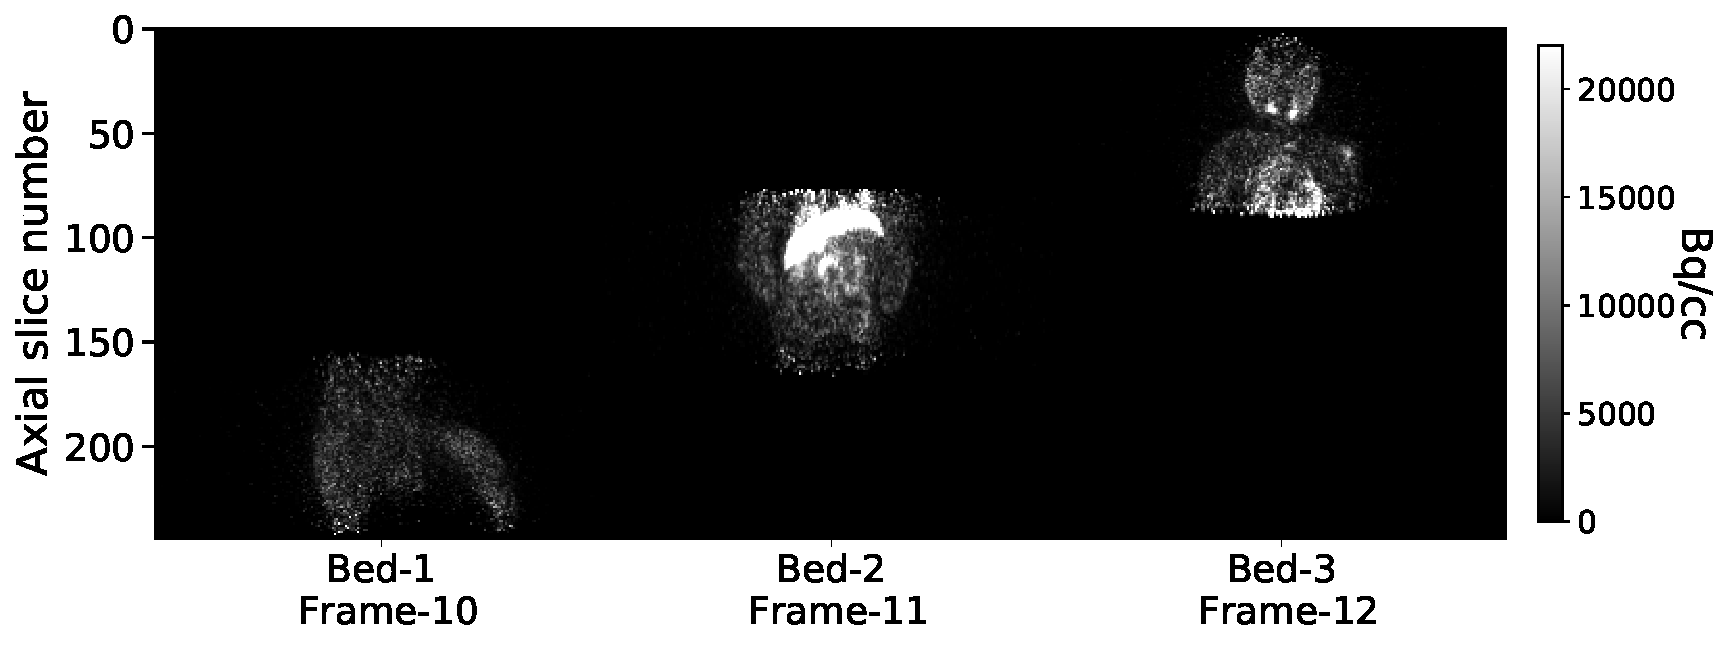
\includegraphics[scale=0.5,angle=0]{3_Results/3_3_DWB_Reconstruction/figures/Macaque_3D.pdf}
\caption{Example three frame images from a three bed DWB acquisition.} 
\label{fig_3_3:Macaque}
\end{figure} 
%
\begin{figure} [h!]
%\centering
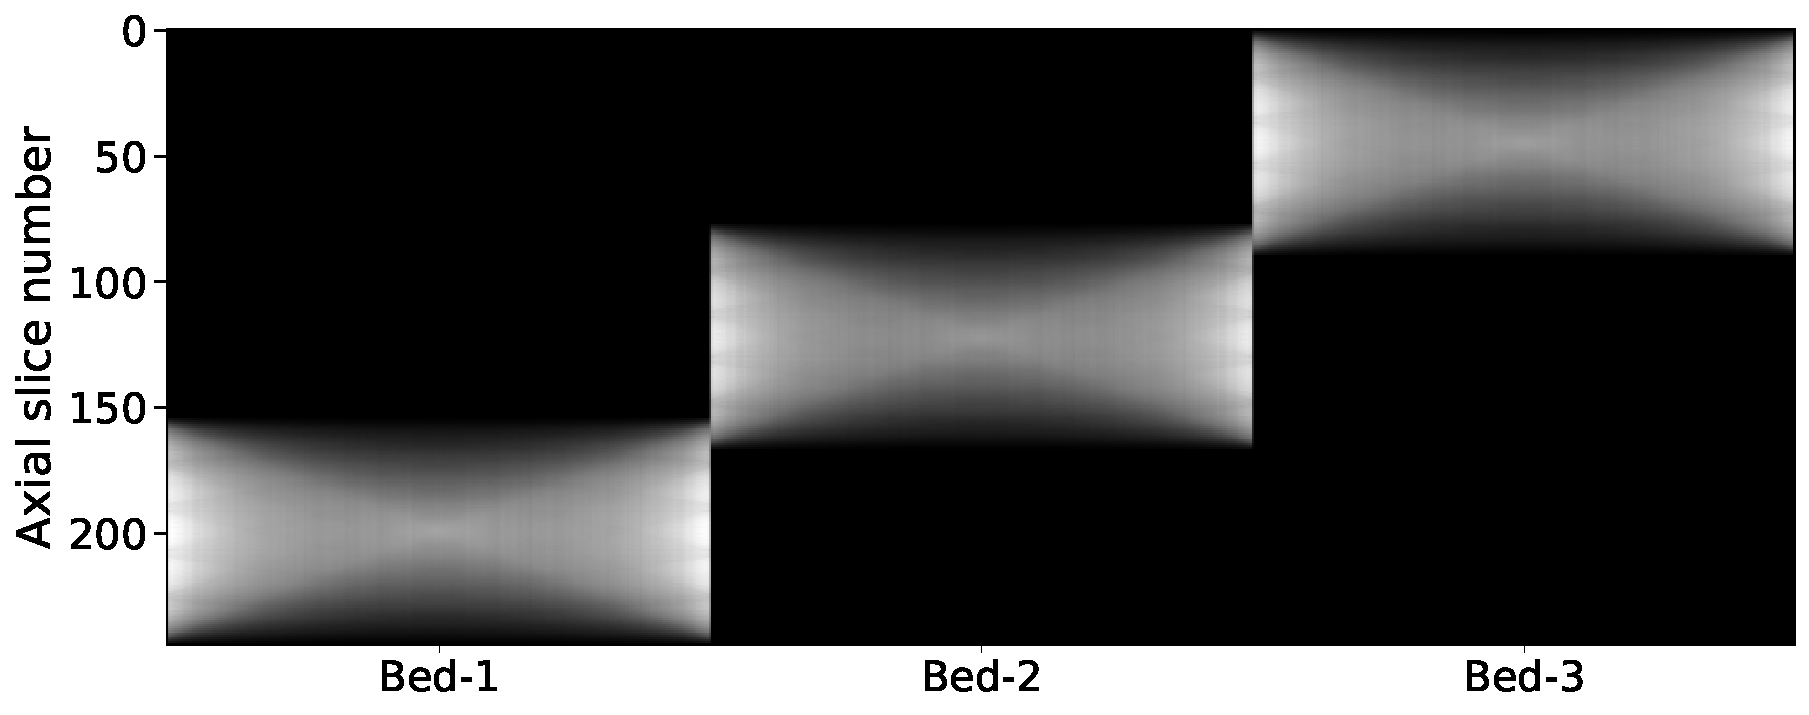
\includegraphics[scale=0.42,angle=0]{3_Results/3_3_DWB_Reconstruction/figures/Macaque_Sensitivity.pdf}
\caption{Example three frame sensitivity images from a three bed positions DWB acquisition.} 
\label{fig_3_3:Macaque_Sensitivity}
\end{figure} 
%
In addition to DWB data alone, the described methodology for direct multi-bed dynamic reconstruction allows for any sequence of the acquired bed/frames to be used within the iterative reconstruction loop. Furthermore, the use of the DSB dataset can also be included in the iterative loop, while also being sub-divided into multiple short frames.

\subsection{Dynamic reconstruction: nested optimization for DWB datasets}
As described previously, dynamic reconstruction is often performed using the nested optimization framework, to accelerate convergence~\cite{Wang2010,Matthews2010}.
Some additional considerations need to be made prior to the use of this multi-bed dynamic reconstruction framework with nested otpimization.

The nested optimization framework decouples the tomographic update process over the PET data from the dynamic model fitting process on image space. The two steps are conducted respectively with an MLEM update over the PET raw data using equation~\ref{eqn:EM_Update_image} to get an individual EM update image for each frame, followed by kinetic model fitting which optimises the likelihood function of equation~\ref{eqn:NestedOptimization}. 

For single bed dynamic data the sensitivity term of the likelihood function over image space can be ignored, assuming that it is constant over time for each voxel, and the likelihood function can be optimised using an image based EM update over image space with equation~\ref{eqn:NestedEM}~\cite{Wang2010,Reader2014}.

In the case of DWB data and overlapping bed positions the sensitivity term has to be maintained, as its value will change with different frames for voxels in the overlapping regions.
Thus the two step process, for direct multi-bed dynamic reconstruction with nested optimization, can be written as

\begin{equation}
\label{eq3_3:NestedMultibed}
\text{}
\begin{cases}  
f_{tj}^{(\textrm{EM})}(\bm\theta^{(k)}) = \frac{f_{tj}(\bm\theta^{(k)})}{\sum_{i=1}^{n_i} P_{tij}} 
\sum_{i=1}^{n_i} P_{tij} 
\frac{y_{ti}}{\sum_{d=1}^{n_j} P_{tid} f_{td}(\bm\theta^{(k)}) + C_{ti} } \\ \\
\argmax{\bm{\theta}} 
\sum_{t=1}^{n_t} \sum_{b=1}^{n_j} \left[ \sum_{i=1}^{n_i}  P_{tib} \right]
\left[ -f_{tb}(\bm\theta^{(k)}) + 
ln( f_{tb}(\bm\theta^{(k)})) 
f_{tb}^{(\mathrm{EM})}(\bm{\theta}^{(k)})
\right] .\\
\end{cases}
\end{equation}

The tomographic update of this two-step optimization process is effectively an update over the DWB data for independent frame reconstruction, followed by an image space optimization process that now needs to consider the sensitivity $\sum_{t=1}^{n_t} \sum_{i=1}^{n_i}  P_{tib}$ of each time point $t$ in the TAC of each voxel $j$. For linear models, where before an image based MLEM algorithm was used for this image space optimization process, an weighted MLEM update can be used with the sensitivity of each time point $t$ as the weight. Alternatively, for linear and non-linear models LS based optimization algorithms can be used with the addition of the the sensitivity value as weight.
%
\iffalse 
\begin{equation}
\theta_j^{(k+1)} = \frac{\theta_j^{(k)}}
{\sum_{p=1}^{n_p} w B_{pj}}
\sum_{p=1}^{n_p} w B_{pj} 
\frac{f_{j}^{(EM)}(\bm{\theta}^{(k)})}{\sum_{d=1}^{n_j} B_{pd}\theta_d^{(k)} } \\.
\label{eqn3_3:WeightedNestedEM}
\end{equation}
\fi
%
\subsection{Real Data}
Two DWB scans from the IsotoPK study were used for assessing the described direct multi-bed dynamic reconstruction method. Both scans were conducted on a single volunteer in a single day, without and with the use of the inhibitor (rifampicin) respectively.The two scans will be refereed to as \textit{CTRL} and \textit{RIF} scans, standing for control and rifampicin. The volunteer was a male (25y) weighting 66Kg on the examination day. The two dynamic scans were conducted with injection of 141.53 MBq and 90.77 MBq of [$^{11}$C] Glyburide respectively. The first scan was conducted with 14 WB passes, with 9$\times$20, 5$\times$30 s frames per bed position. The second scan included 15 WB passes, with 9$\times$20, 6$\times$30 s frames per bed position. Both scans begin with an 180 s DSB acquisition centered over the liver, starting at the time of injection, before the DWB acquisition. By splitting the DSB into 18x10 s frames and considering each Step and Shoot acquisition as an individual frame, the two scans resulted in a total of 88 and 93 frames respectively. 
The planned bed positions are shown in figure~\ref{fig_3_3:IsotoPK_BedPositionsOnMR} for the DSB and DWB phase of the \textit{CTRL} scan. 

The complete \textit{CTRL} and \textit{RIF} datasets, including the DSB and DWB data, were reconstructed within the developed direct multi-bed dynamic reconstruction platform, using an OSEM algorithm with 28 subsets and EM nested optimization of 20 sub-iterations. Both datasets made use of TOF information within the reconstruction. 
As the IsotoPK study is an exploratory pharmacokinetic study, dynamic reconstructions were performed with the spectral model for temporal regularisation of frame activity estimates as well as for the direct estimation of $K_1$ parametric images, without strong assumptions about the underlying kinetics.
Additional dynamic reconstructions were performed for DWB data, without the use of the initial DSB data, to test extrapolation of the spectral model on early (non-sampled) frames. 
A total number of 17 spectral basis functions were used, with $\beta_1 ... \beta_{M-1}$ logarithmically spaced within the range of 3 to 0.001 $min^{-1}$, while including $\beta_0$ and $\beta_{M}$ to account for trapping and blood fraction in the data. Similarly to the simulation study, the assumption of the total blood activity concentration $C_{B}$ being proportional to the arterial blood plasma $C_{P}$ was used in the estimation of the basis functions.
Using the fitted spectral model, the approximate $\boldsymbol{K_1^*}$ parametric images were estimated similar to the methodology used in the simulation study of chapter ~\ref{Chap3_2:SimStudy}.
In addition to the dynamic reconstructions, 3D reconstruction was performed using the same framework and OSEM algorithm with 28 subsets.

Manual arterial blood samples were taken during both scans, to derive the input function and for blood analysis (to measure the metabolites fraction and for plasma binding of the tracer). The measured input functions were linearly interpolated and then used in the estimation of the spectral basis functions. 

\begin{figure} [h!]
\centering
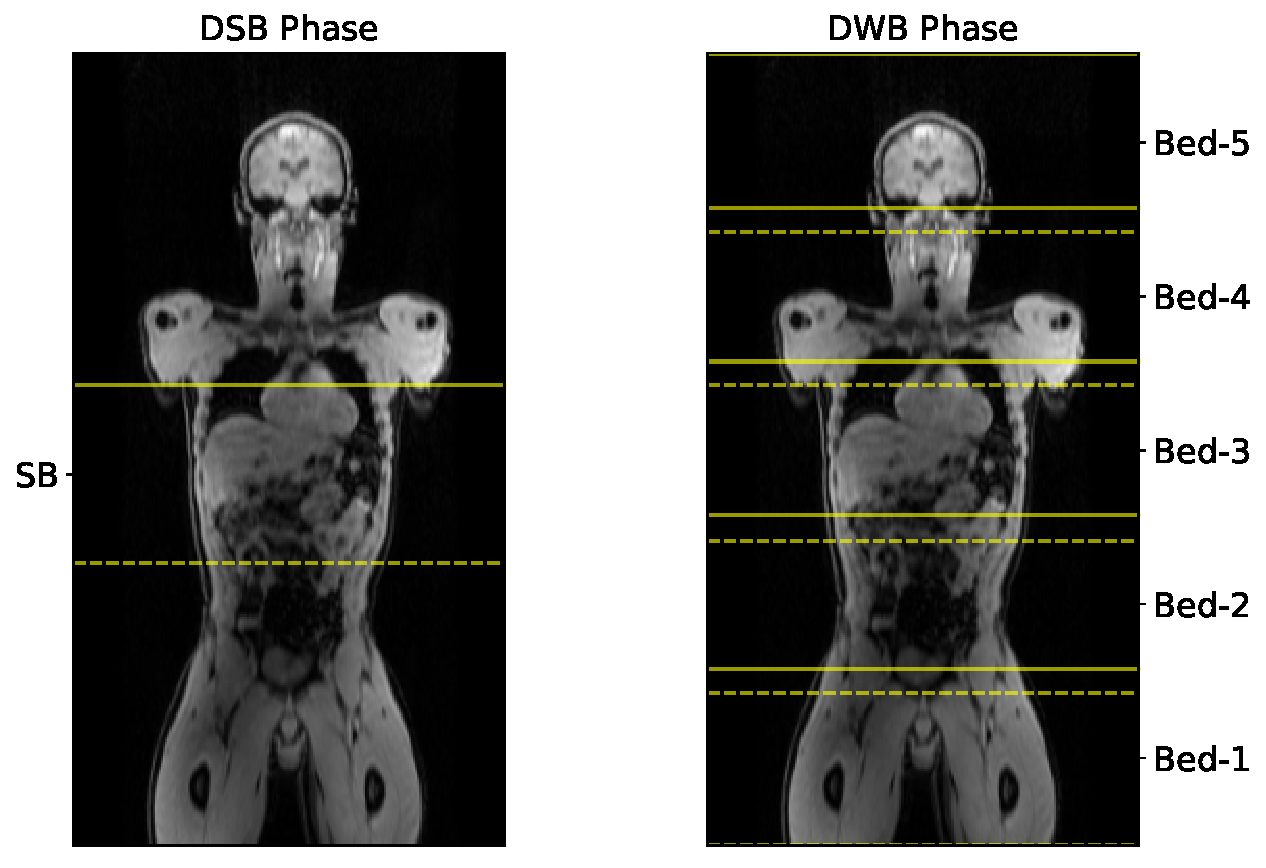
\includegraphics[scale=0.42,angle=0]{3_Results/3_3_DWB_Reconstruction/figures/3_3_IsotoPK_CTRL_PositionsOnMR.pdf}
\caption{Planned DSB and DWB bed positions shown on coronal MRAC image, with bed start (\protect\tikz[baseline]{\protect\draw[line width=0.5mm] (0,.8ex)--++(1,0) ;}) and end (\protect\tikz[baseline]{\protect\draw[line width=0.5mm,densely dashed] (0,.8ex)--++(1,0) ;}) positions.} 
\label{fig_3_3:IsotoPK_BedPositionsOnMR}
\end{figure} 

The VOIs listed in table~\ref{tab:IsotoPK_VOIs}  were drawn manually to and used to validated and compare the reconstruction methods.
The 
\begin{table}[h!]
\centering
\caption{\label{tab:IsotoPK_VOIs} VOIs used for evaluation of DWB scans.}
\begin{tabular}{lll}
\toprule
\textbf{VOI Name} & \textbf{Availability in Data}  \\
\midrule
Brain        & DWB                 \\
Myocardium & DSB \& DWB              \\
Left Ventricle (LV) & DSB \& DWB     \\
Left Kidney (Kidney$_\mathrm{L}$) & DSB \& DWB  \\
Right Kidney (Kidney$_\mathrm{R}$) & DSB \& DWB \\
Spleen & DSB \& DWB \\
Liver  & DSB \& DWB \\
Aorta & DSB \& DWB \\
Bladder & DWB \\
Leg Muscle & DWB \\
\toprule
\end{tabular}
\end{table}

\subsubsection{Liver dual-input function simulation}
For the liver which is one the main organs of interest in the IsotoPK study, as discussed in section~\ref{liver_PV_theory}, the dual input function model is necessary for accurate modeling of tracer behaviour. 
When this is not accounted for, parametric estimates derived from single input function models are expected to be biased.  
A toy simulation was conducted to study how quantification of $K_1^{*}$ is affected by the use of the spectral model with a single input function and to study whether relative differences of true underlying $k_1$, such as those expected from the comparison of the \textit{CTRL} to the \textit{RIF} scan, can still be accurately deduced using the spectral model deduced $K_1^{*}$.

\section{Results}
\subsection{Comparison between 3D and 4D spectral reconstruction on DWB data}
Coronal \gls{mip} images of 3D reconstructions from the \textit{CTRL} scan are shown in figure~\ref{fig_3_3:IsotoPK_CTRL_DSB_3D} and figure~\ref{fig_3_3:IsotoPK_CTRL_DWB_3D}, for a late frame of the DSB acquisition and early frames of the DWB acquisition respectively. 
Similarly, \gls{mip} images of 4D spectral reconstruction of the \textit{CTRL} scan are shown in figure~\ref{fig_3_3:IsotoPK_CTRL_DSB_4D} and figure~\ref{fig_3_3:IsotoPK_CTRL_DWB_4D} for the same respective frames. 
As the spectral model is applied on the image space of the entire effective FOV, the 4D reconstruction results in frame images that are estimated from the fitted model of the entire FOV. As such, activity estimates of locations that are not sampled for a given frame within the DWB scan are interpolated from the frame data of the entire DWB scan. For the frames of the DSB scan, locations that are not sampled by the single bed acquisition have activity estimates that are extrapolated from the fitted spectral model of later frames.

\begin{figure} [h!]
\centering
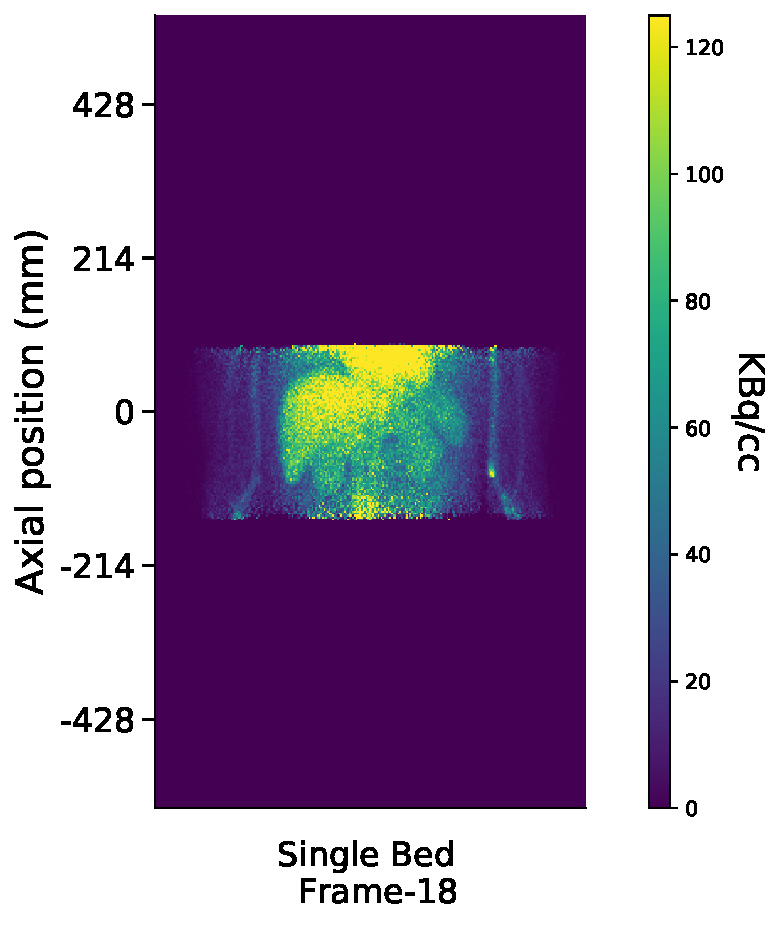
\includegraphics[scale=0.52,angle=0]{3_Results/3_3_DWB_Reconstruction/figures/3_3_IsotoPK_CTRL_DSB_3D.pdf}
\caption{Coronal MIP image of 3D reconstruction (4it28sub) of a single frame from the DSB acquisition on the \textit{CTRL} scan}
\label{fig_3_3:IsotoPK_CTRL_DSB_3D}
\end{figure} 

\begin{figure} [h!]
\centering
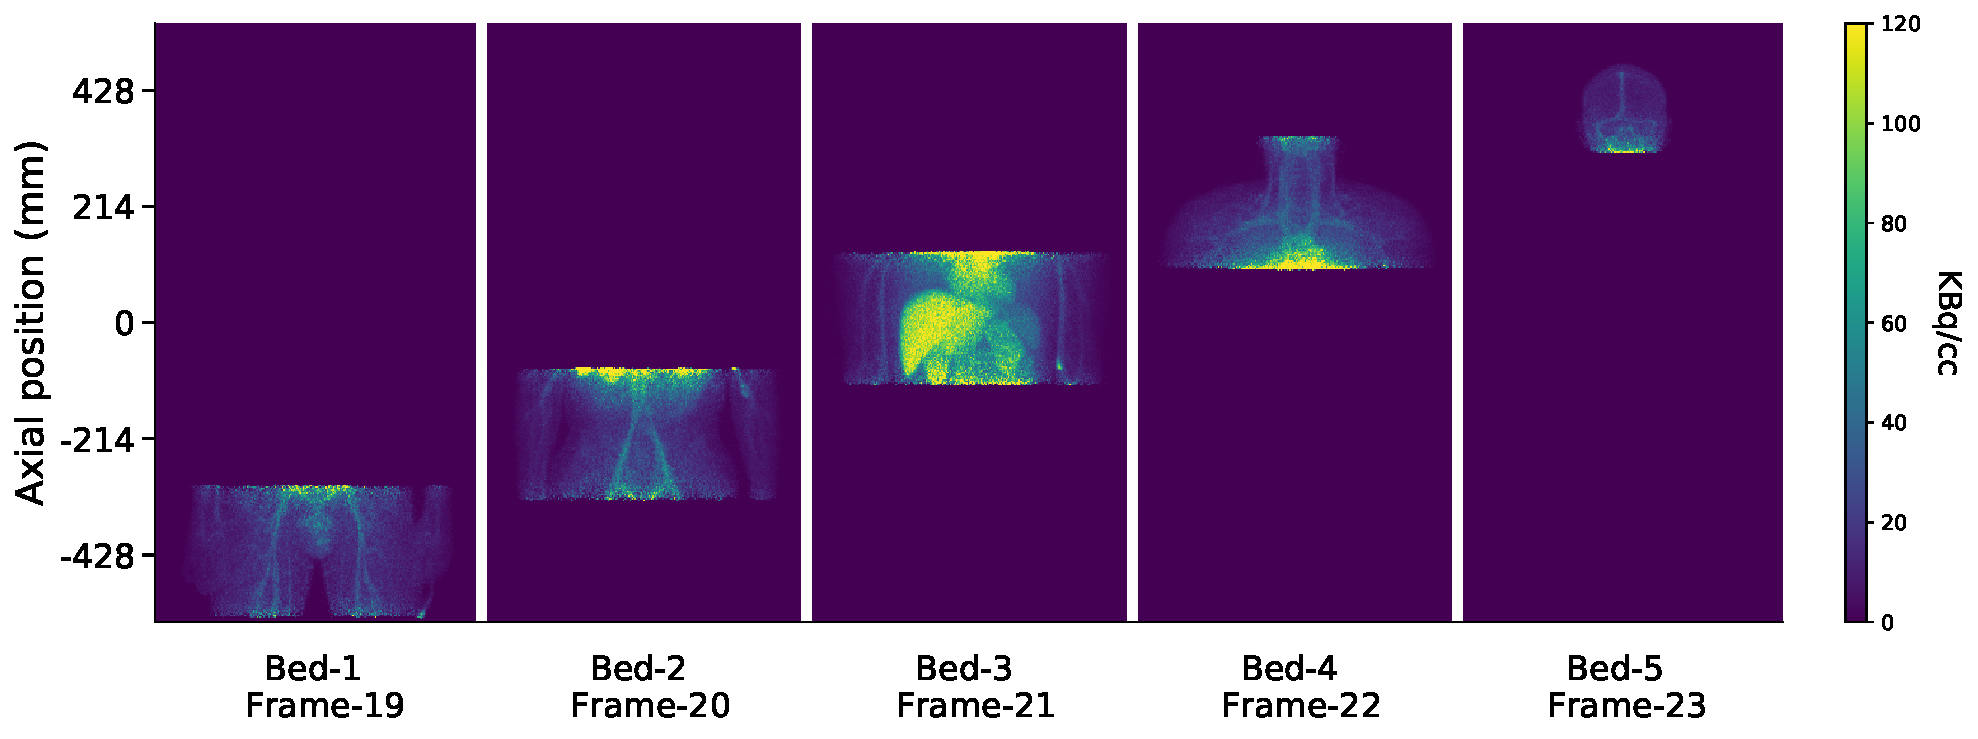
\includegraphics[scale=0.52,angle=0]{3_Results/3_3_DWB_Reconstruction/figures/3_3_IsotoPK_CTRL_DWB_3D.pdf}
\caption{Coronal MIP images of 3D reconstructions (4it28sub) of a single frame per bed position from the first whole-body pass of the DWB acquisition on the \textit{CTRL} scan.}
\label{fig_3_3:IsotoPK_CTRL_DWB_3D}
\end{figure} 

\begin{figure} [h!]
\centering
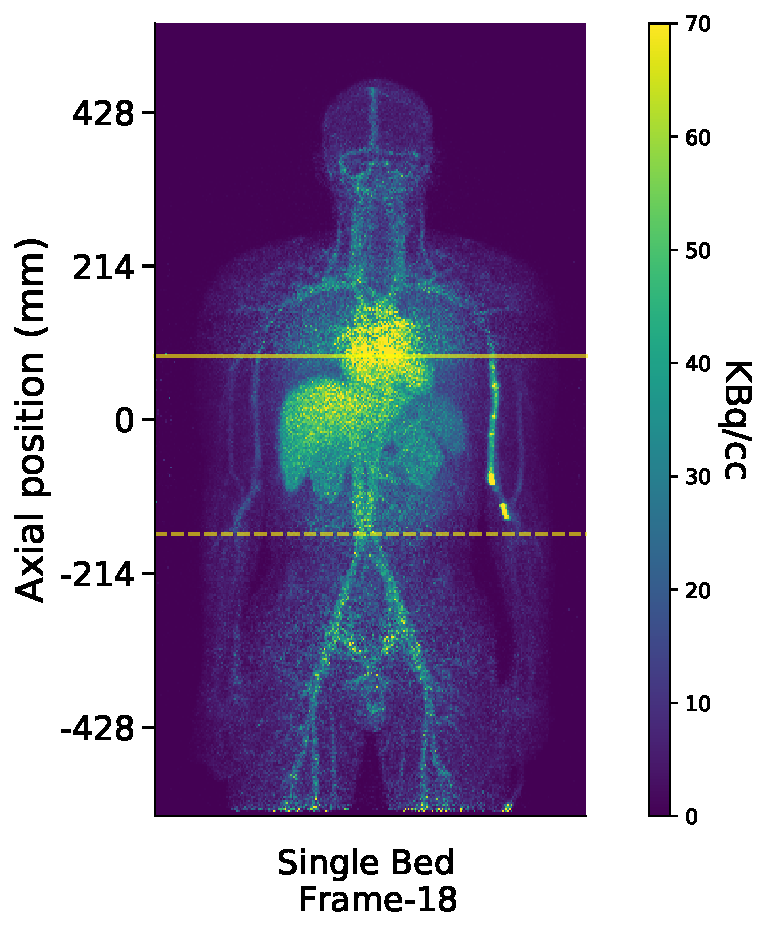
\includegraphics[scale=0.52,angle=0]{3_Results/3_3_DWB_Reconstruction/figures/3_3_IsotoPK_CTRL_DSB_4D.pdf}
\caption{MIP image of a single frame from 4D reconstruction (15it28sub) of the CTRL scan}
\label{fig_3_3:IsotoPK_CTRL_DSB_4D}
\end{figure} 

\begin{figure} [h!]
\centering
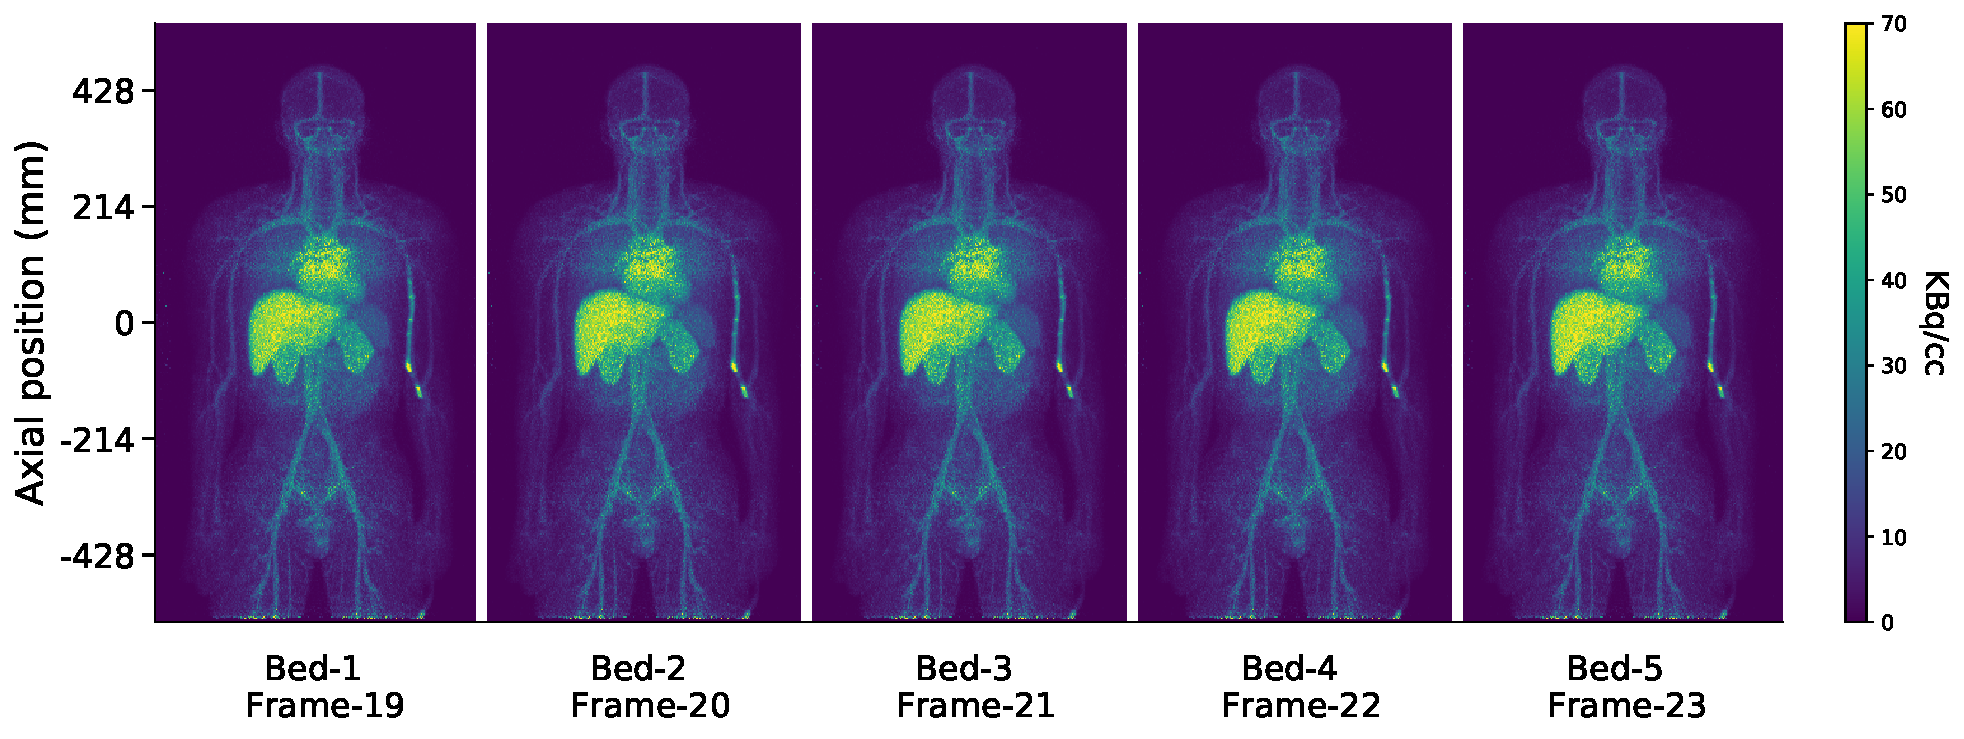
\includegraphics[scale=0.52,angle=0]{3_Results/3_3_DWB_Reconstruction/figures/3_3_IsotoPK_CTRL_DWB_4D.pdf}
\caption{MIP image of the first whole-body pass frames from 4D reconstruction (15it28sub) of the CTRL scan.}
\label{fig_3_3:IsotoPK_CTRL_DWB_4D}
\end{figure} 

Plots of mean VOI activity against iteration, for early and late frames, over the liver and the leg muscle VOI were used to evaluate at which iteration the mean values begin to stabilise. These plots are shown in figure~\ref{fig_3_3:IsotoPK_CTRL_DWB_4D_Convergence} and figure~\ref{fig_3_3:IsotoPK_CTRL_DSB_3D_Convergence} of the appendix~\ref{chap:AppendixC}. For 4D spectral reconstruction the evaluated mean values showed relatively stable behaviour from the 15th iteration onwards, which was chosen for subsequent comparisons of reconstructions. For 3D reconstruction mean values did not show stable behaviour in both regions within the first 8 iterations and the 4th iteration was chosen in subsequent comparisons as a comprise between reliability of mean values convergence and image noise.  

TACs of the evaluated VOIs are plotted in figure~\ref{fig_3_3:IsotoPK_CTRL_DWB_4D_vs_3D_Central} and~\ref{fig_3_3:IsotoPK_CTRL_DWB_4D_vs_3D_Peripheral}, for VOIs sampled in both DSB and DWB acquisitions and for VOIs sampled only during the DWB acquisition respectively. In figure~\ref{fig_3_3:IsotoPK_CTRL_DWB_4D_vs_3D_Peripheral} the time point of the start of the DWB acquisition is indicated by the red dotted line.
As already mentioned, the 4D spectral reconstruction results in an activity estimate of every location of the image for every frame of the study, while 3D reconstruction results in activity estimates for the sampled frames only at each location. This is why the TACs from the 4D reconstruction of the \textit{CTRL} data show a total of 88 frame points for all VOIs and a total of 32 frame points (18 from DSB plus 14 from DWB) for regions included in the DSB acquisition and only 14 frames for regions seen solely by the DWB acquisition. 

For the VOIs seen by both DSB and DWB acquisitions the TACs between 3D and 4D spectral reconstruction are in good agreement for all evaluated VOIs, as seen in~\ref{fig_3_3:IsotoPK_CTRL_DWB_4D_vs_3D_Central}. For the brain and muscle VOIs seen by the DWB acquisition alone there is a relatively good agreement, with slight overestimation in early frames of the brain region and underestimation on later frames as seen in~\ref{fig_3_3:IsotoPK_CTRL_DWB_4D_vs_3D_Peripheral}. By contrast, at the bladder VOI there is a strong mismatch of the 3D and 4D spectral reconstruction, with the 3D reconstruction showing clearly the bladder filling process and the 4D spectral reconstruction showing an increasing behaviour produced by the exponential functions. 

A look into the VOI means of the spectral parametric images is given in the appendix material, where it is seen that the component of full trapping $\phi_0$ is strongly used in the bladder region, in an attempt to fit the underlying process. But the use of the input function and the decaying exponentials is not enough to fit this process. Further considerations to this issue are addressed in the section~\ref{sub_section:residuals}.

\begin{figure} [h!]
\centering
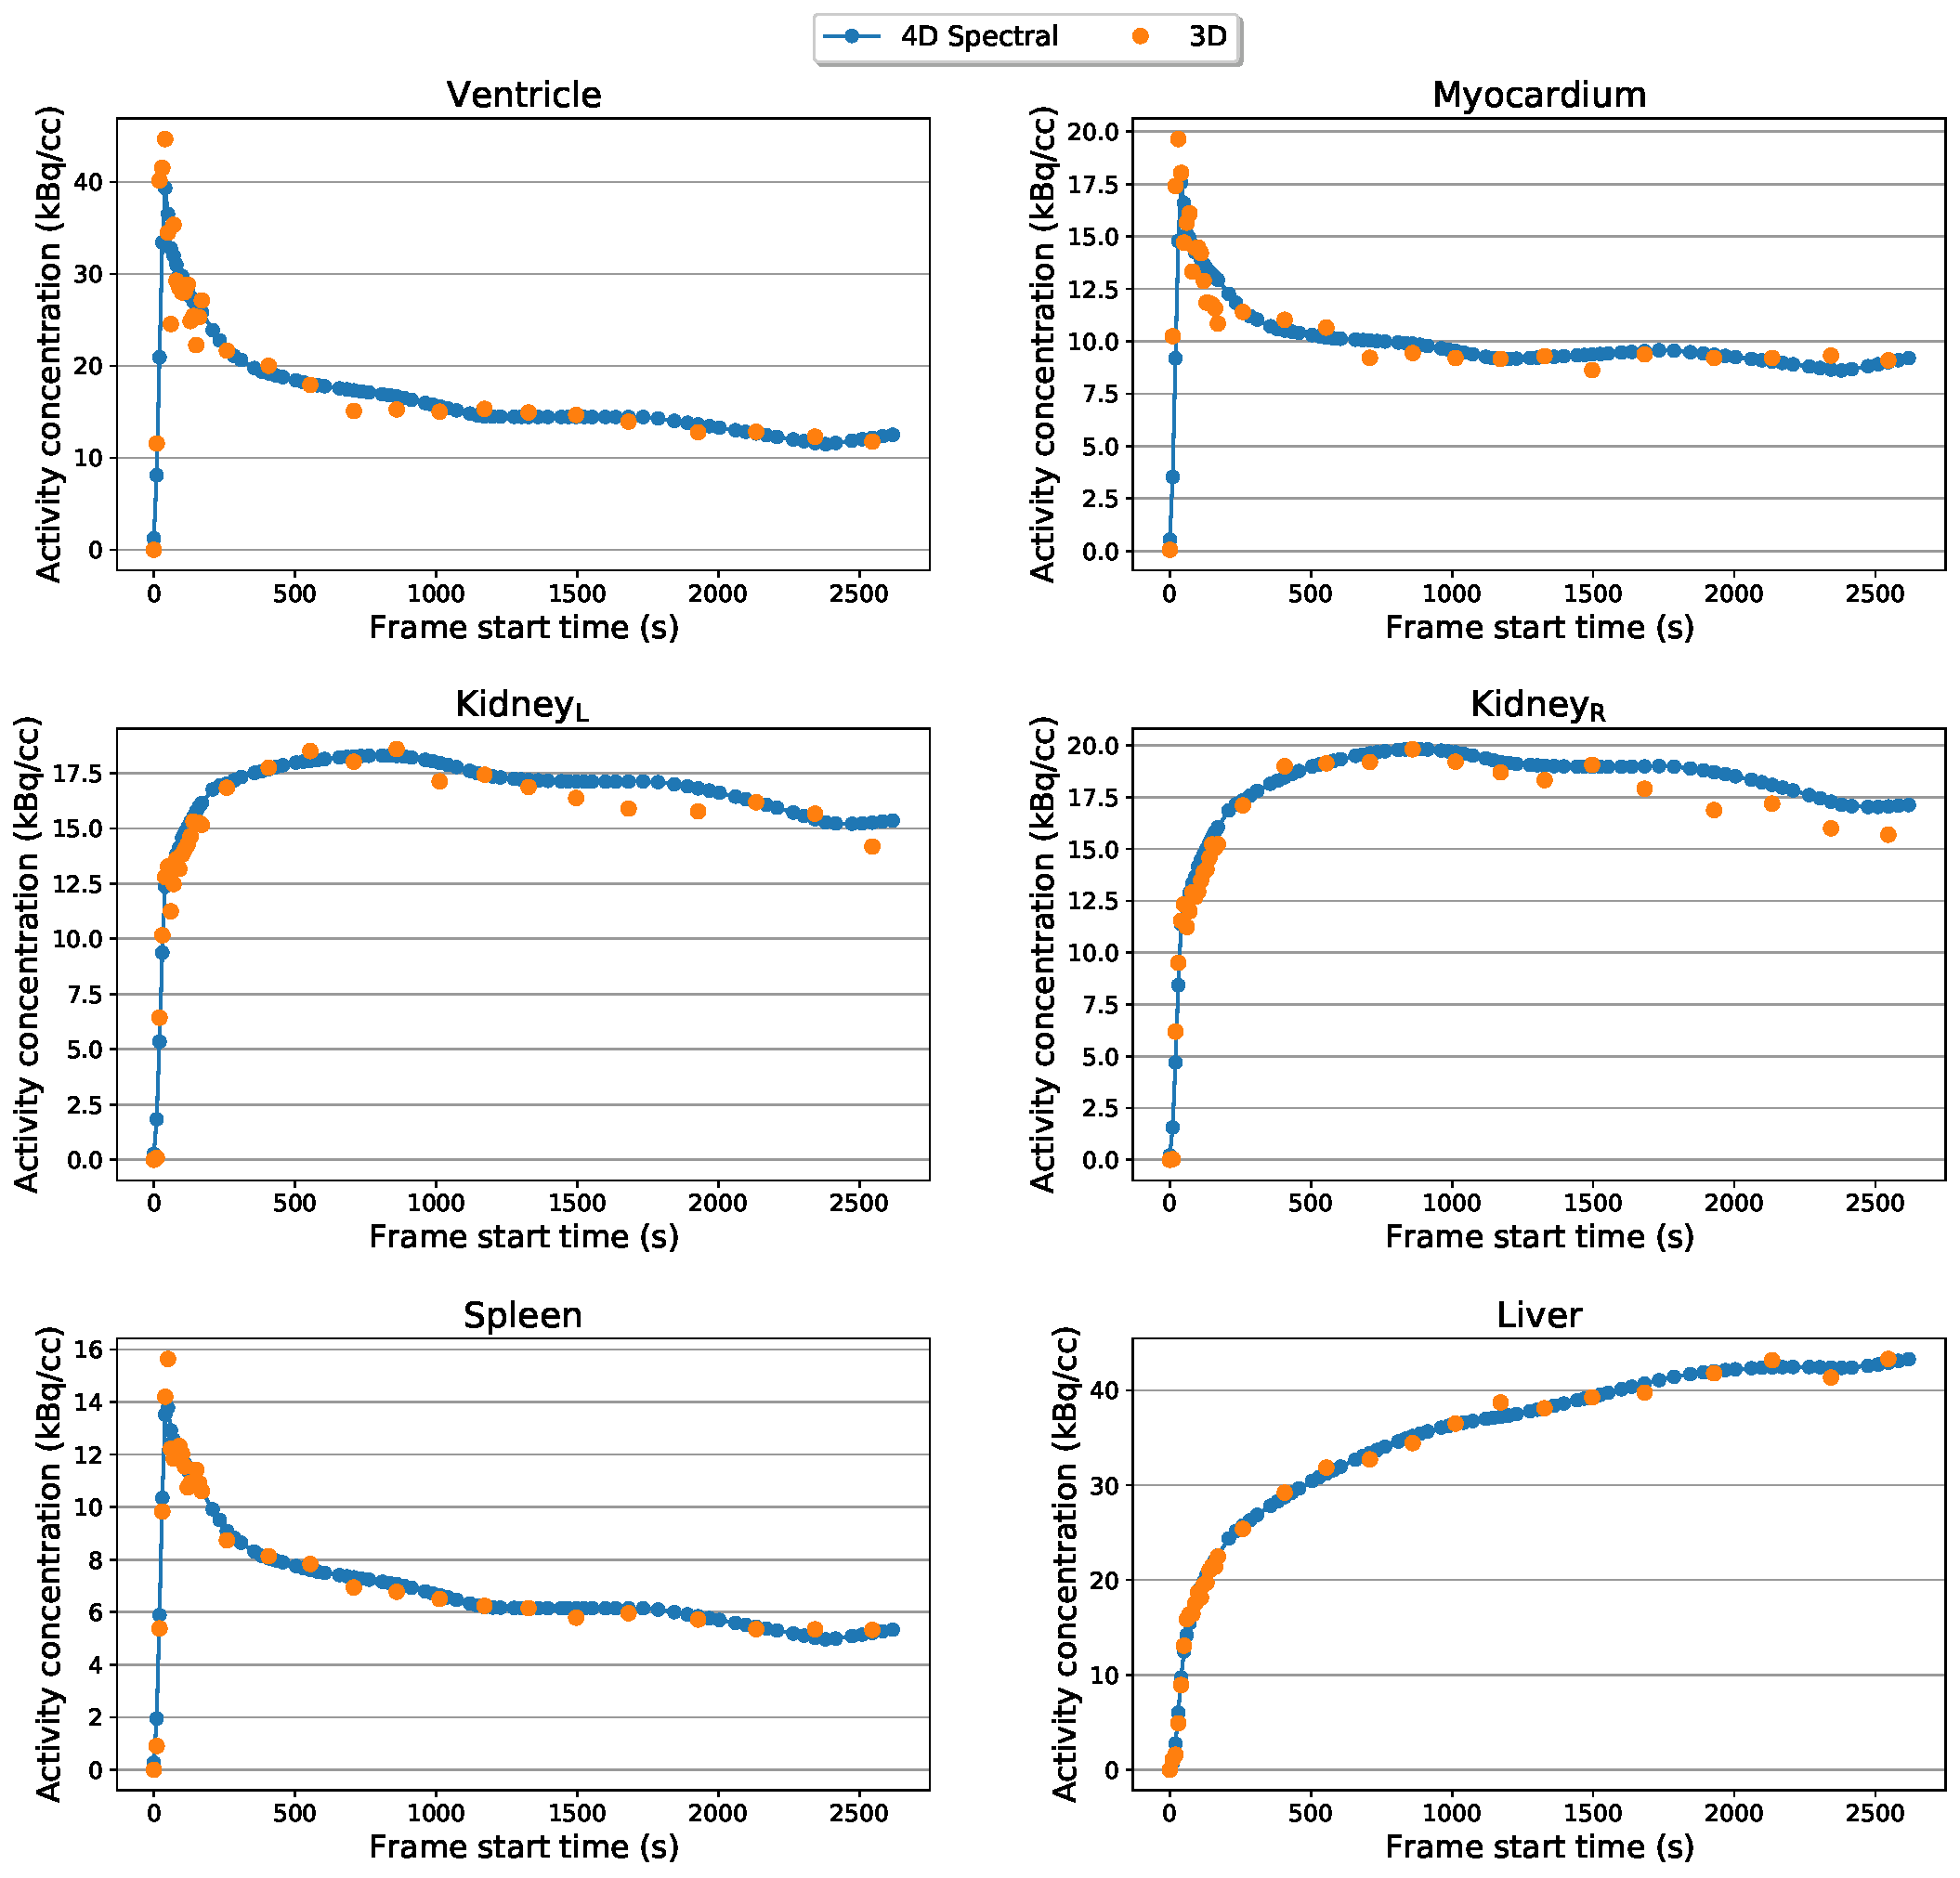
\includegraphics[scale=0.5,angle=0]{3_Results/3_3_DWB_Reconstruction/figures/3_3_IsotoPK_CTRL_DWB_3D_vs_4D_central.pdf}
\caption{VOI mean time activity curves for 3D and 4D spectral reconstruction. VOI regions shown which are included in both DSB and DWB acquisition.}
\label{fig_3_3:IsotoPK_CTRL_DWB_4D_vs_3D_Central}
\end{figure}

\begin{figure} [h!]
\centering
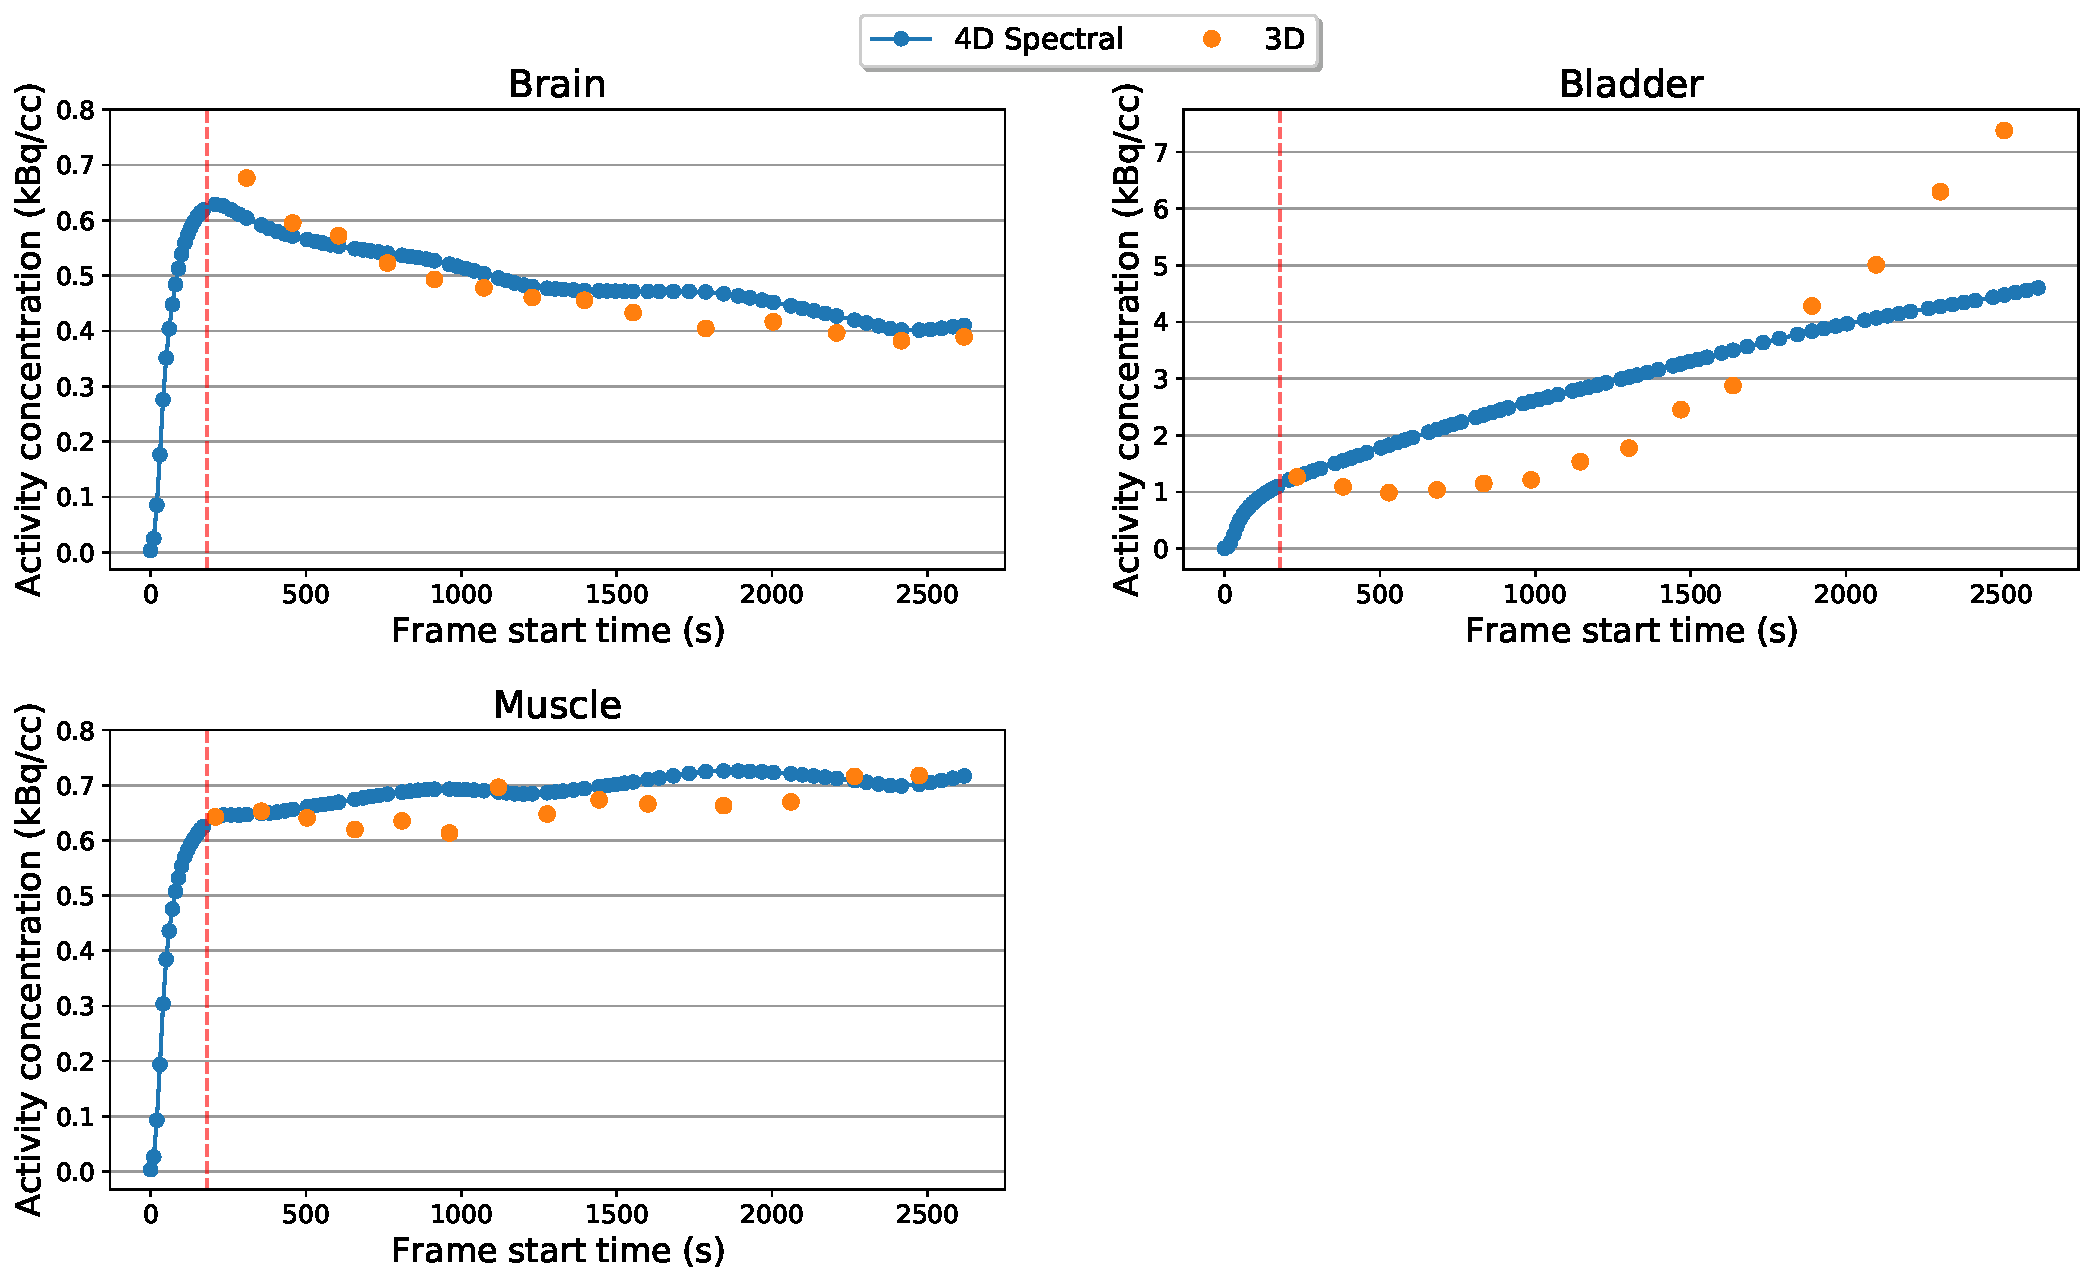
\includegraphics[scale=0.5,angle=0]{3_Results/3_3_DWB_Reconstruction/figures/3_3_IsotoPK_CTRL_DWB_3D_vs_4D_peripheral.pdf}
\caption{VOI mean time activity curves for 3D and 4D spectral reconstruction. VOI regions shown which are covered only by the DWB acquisition, whose start time is designated with a vertical dotted line.}
\label{fig_3_3:IsotoPK_CTRL_DWB_4D_vs_3D_Peripheral}
\end{figure} 

\subsection{Comparison of 4D Spectral reconstruction on DWB data, with and without the use of DSB data}
A comparison between 4D spectral reconstruction with and without the use of the initial DSB data is made in figure~\ref{fig_3_3:IsotoPK_CTRL_DWB_4D_vs_4D_Central} for VOIs covered by both DSB and DWB acquisitions. These show a good agreement of the two spectral reconstructions, with a consistent slight error in the early frame estimations of the reconstruction without use of DSB data, that is relatively small compared to the mean activity of each VOI (maximum of 12.7\% error seen in Spleen VOI). A very good agreement is seen on the liver between the two reconstructions.

The extrapolation of the fitted spectral model from DWB data alone can be made for the early non sampled frames. These show a sharp drop of the fitted TACs, indicating the inadequacy of the used data for extrapolation of the fast early frame behaviour and the cause for the systematic mismatch at early frames of the DWB acquisition.

\begin{figure} [h!]
\centering
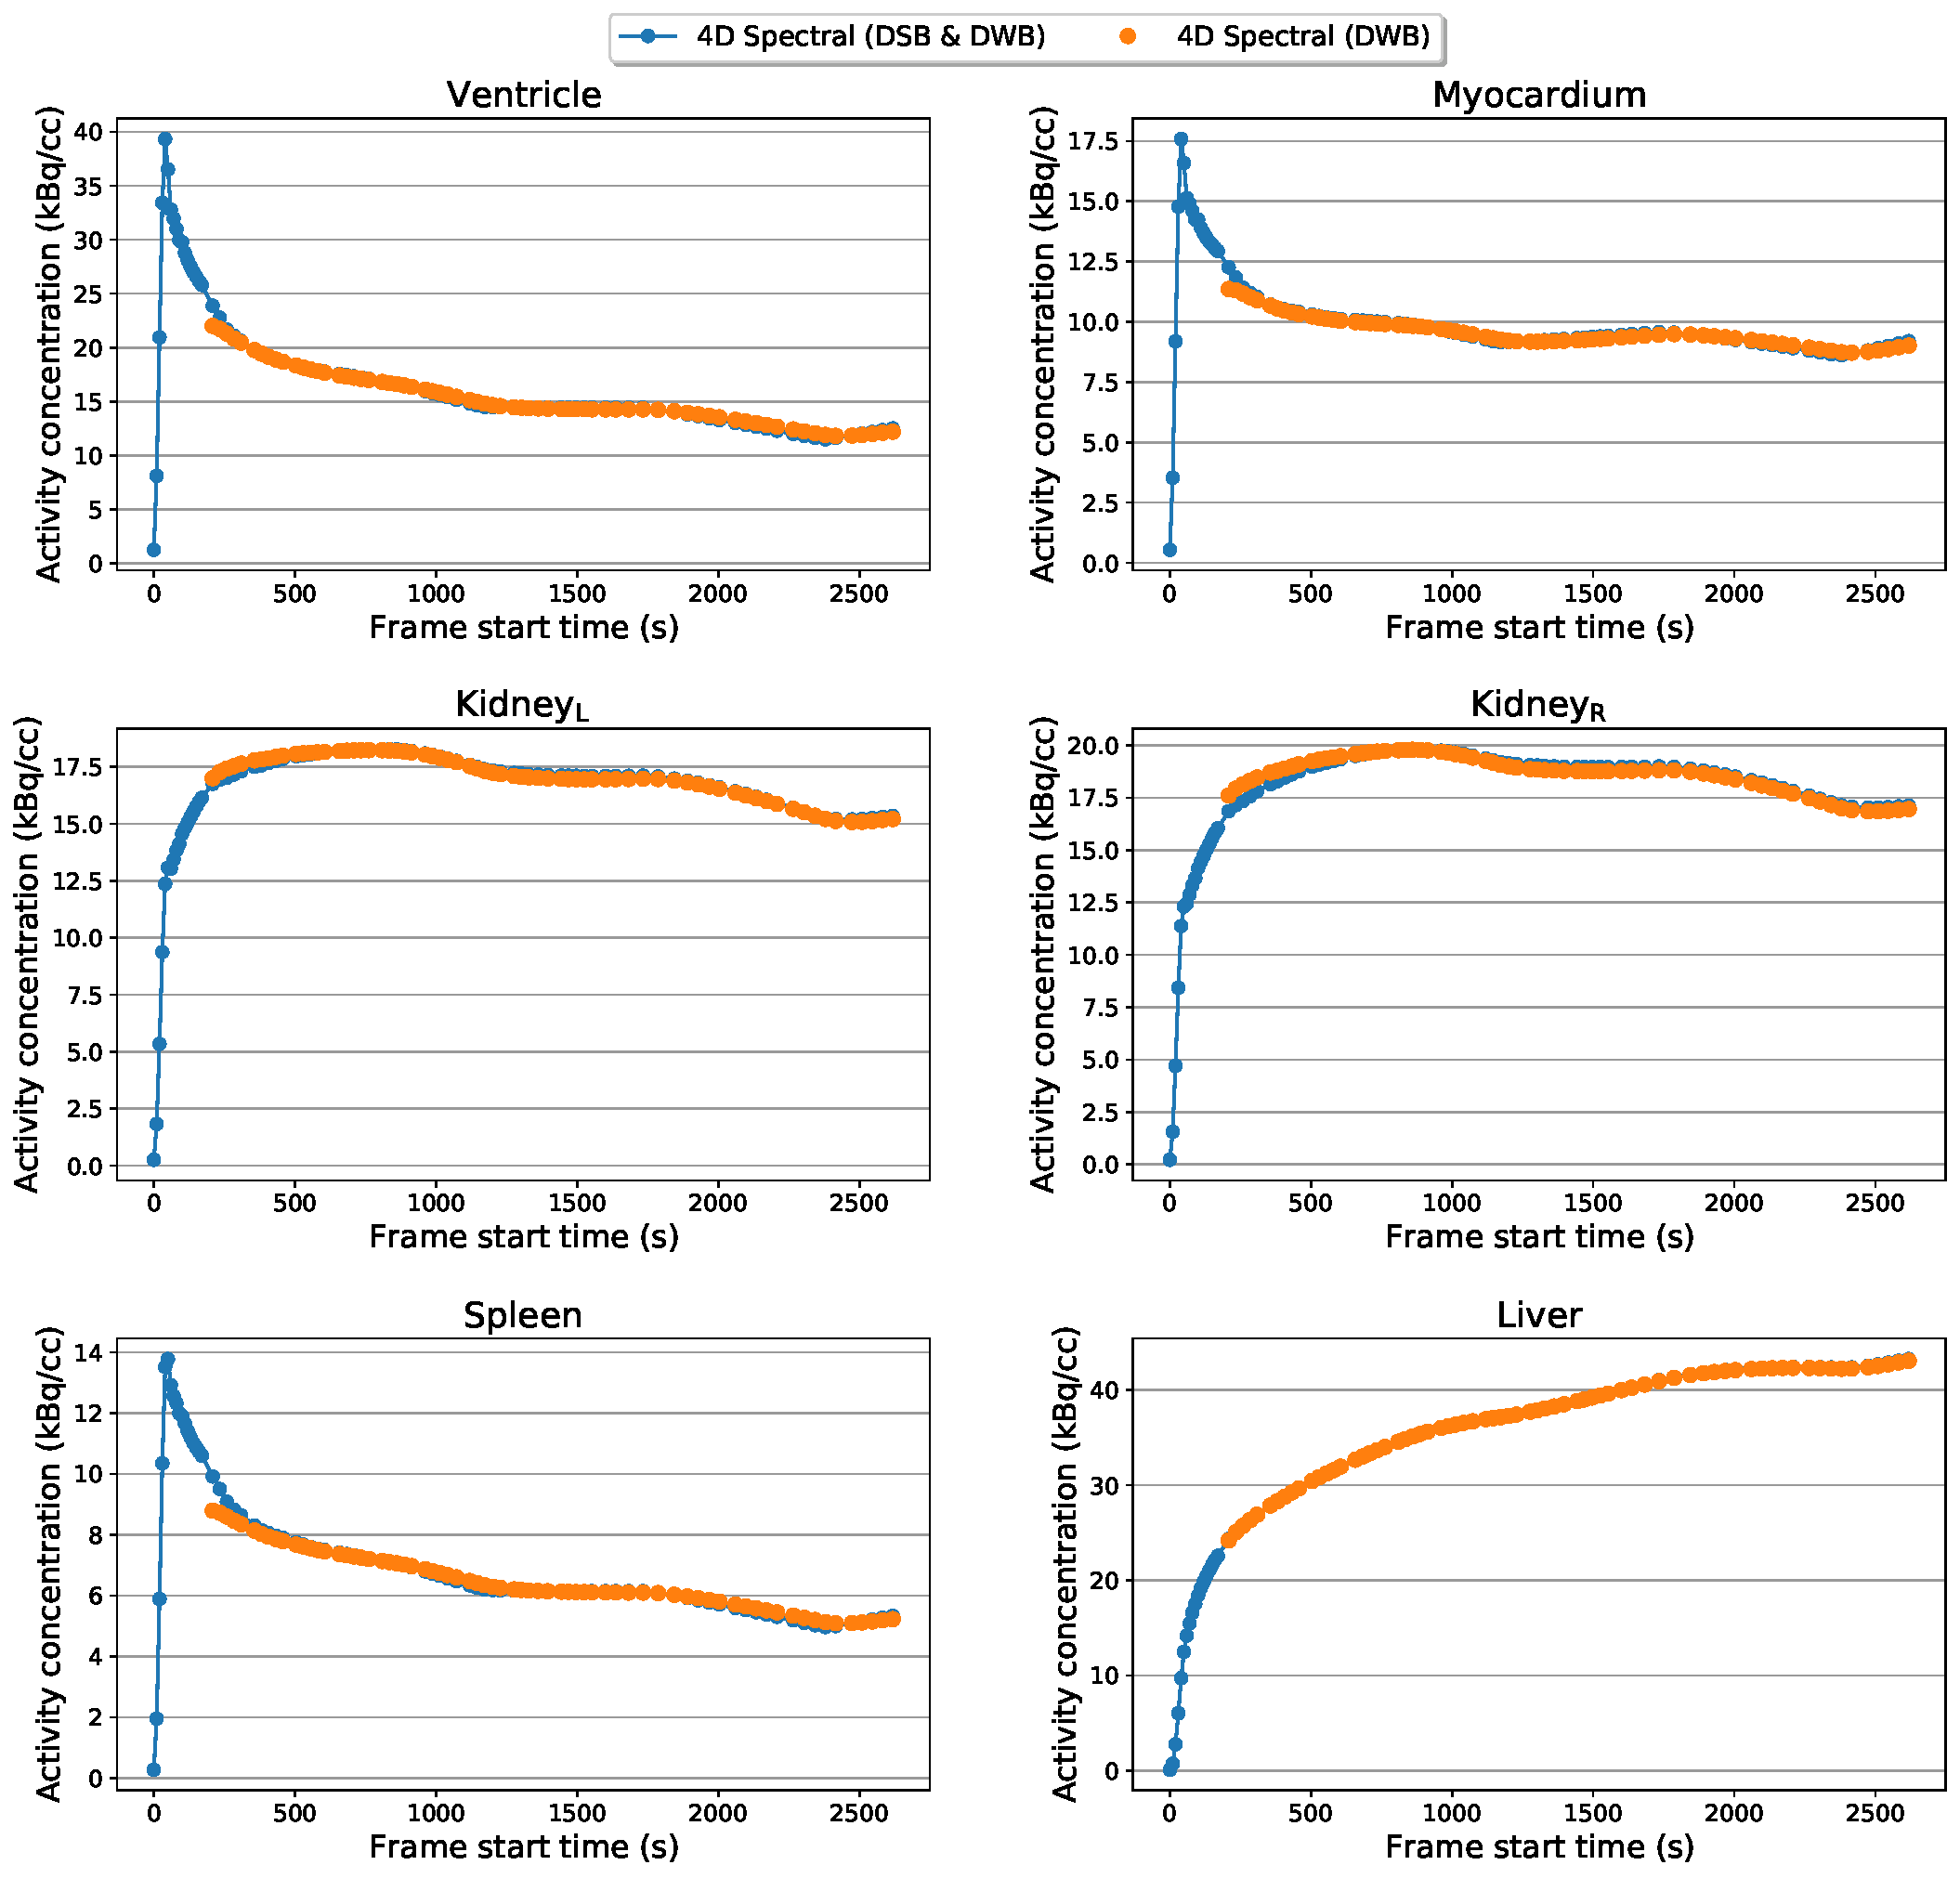
\includegraphics[scale=0.5,angle=0]{3_Results/3_3_DWB_Reconstruction/figures/3_3_IsotoPK_CTRL_DWB_4D_vs_4D_central.pdf}
\caption{VOI mean time activity curves for 4D spectral reconstructions, with and without the use of DSB data. VOI regions shown are included in both DSB and DWB acquisitions.}
\label{fig_3_3:IsotoPK_CTRL_DWB_4D_vs_4D_Central}
\end{figure} 

\subsection{Direct WB parametric image estimation from 4D Spectral reconstructions}
Using the set of equations~\ref{eqn:AllSpectralEqns} and specifically the equation for the derivation of $K_1$, the parametric maps of $K_1^{*}$ were produced by summation of basis $(\phi_0-\phi_{M-1})$. Similar to the simulation study before, the blood fraction correction was neglected in favour of avoiding voxel-to-voxel division and induction of excessive image noise. The result parametric maps for both \textit{CTRL} and \textit{RIF} scans are shown in figure~\ref{fig_3_3:IsotoPK_K1_MIP} and figure~\ref{fig_3_3:IsotoPK_K1_SingleSlice}, as a \gls{mip} in the coronal plane and as a single coronal slice showing the the liver, kidneys and the spleen.
Mean VOI $K_1^{*}$ values,shown in figure~\ref{fig_3_3:IsotoPK_K1_drop}, show a considerable reduction from the \textit{CTRL} to the \textit{RIF} scan by the administration of the inhibitor prior to the \textit{RIF} scan. 

The results of the dual input simulation study, given in appendix~\ref{chap:AppendixC}, indicate that accurate quantification of $K_1$ (or $K_1^{*}$) in the liver using only the arterial input function as an input is not achievable as expected. 
%But by contrast it did show that the genericity of the spectral model allowed for accurate TAC fitting, similar to the result seen on the liver with the real data. 
But the simulation showed that a relative comparison of spectral model $K_1^{*}$ estimates reflects accurately and linearly the differences differences of the true underlying $K_1$, without explicit need for modeling the dual input function.

\begin{figure} [h!]
\centering
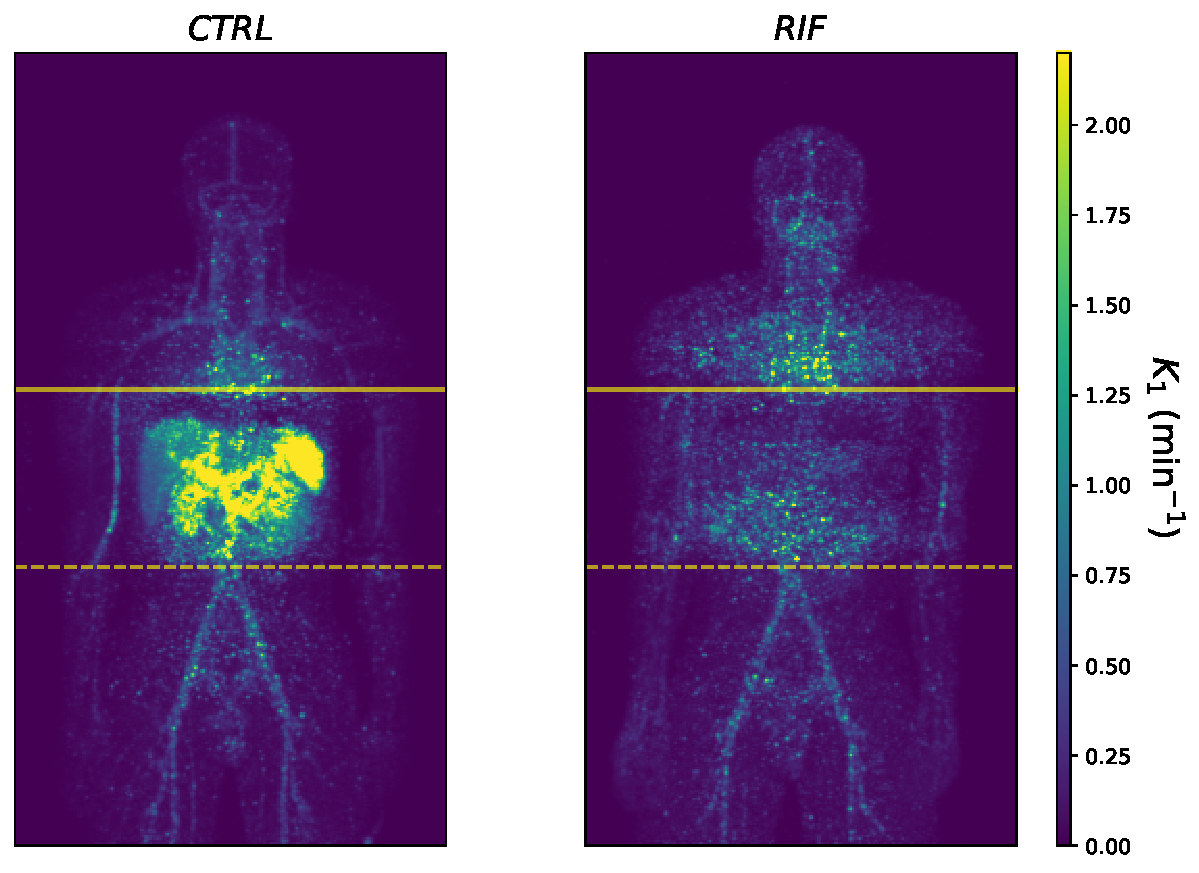
\includegraphics[scale=0.5,angle=0]{3_Results/3_3_DWB_Reconstruction/figures/3_3_IsotoPK_K1_MIPs.pdf}
\caption{$K_1$ MIP images from the 4D spectral reconstruction using both DSB and DWB acquisitions, shown for the \textit{CTRL} and \textit{RIF} scan.}
\label{fig_3_3:IsotoPK_K1_MIP}
\end{figure} 

\begin{figure} [h!]
\centering
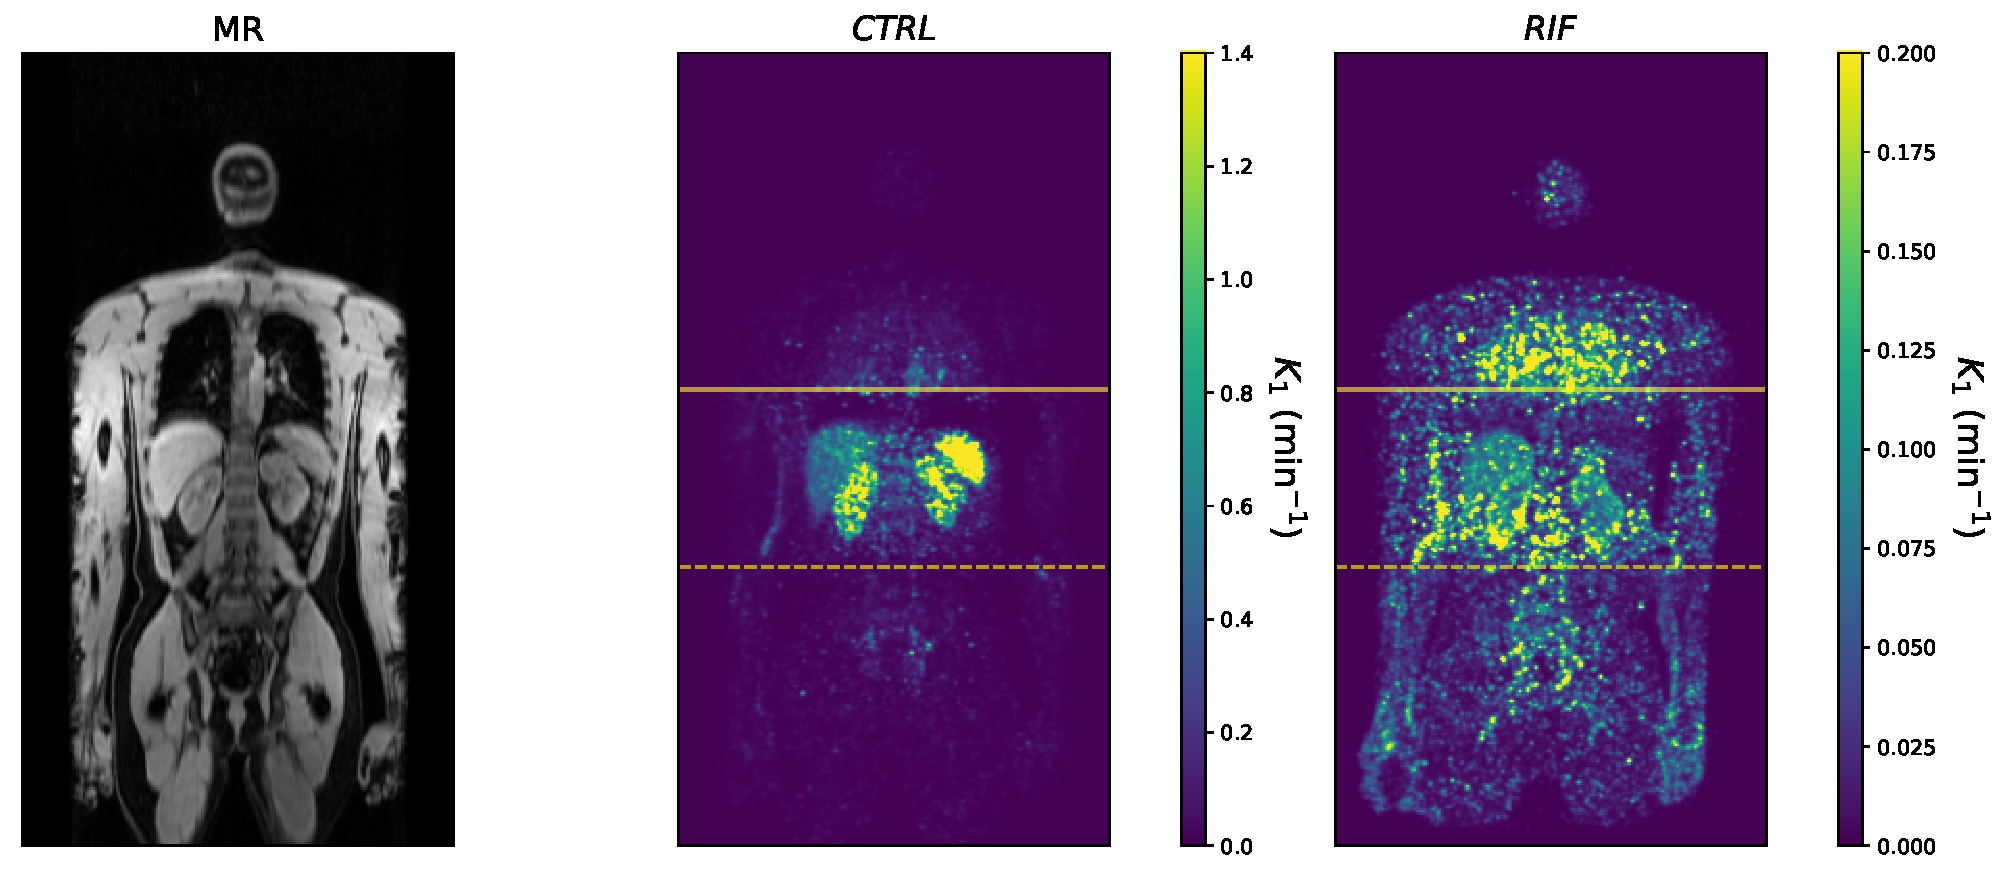
\includegraphics[scale=0.5,angle=0]{3_Results/3_3_DWB_Reconstruction/figures/3_3_IsotoPK_K1_SingleSlice.pdf}
\caption{$K_1^{*}$ values as estimated from the 4D spectral reconstruction for VOI regions included in both DSB and DWB acquisitions , shown for the \textit{CTRL} and \textit{RIF} scan}
\label{fig_3_3:IsotoPK_K1_SingleSlice}
\end{figure} 

\begin{figure} [h!]
\centering
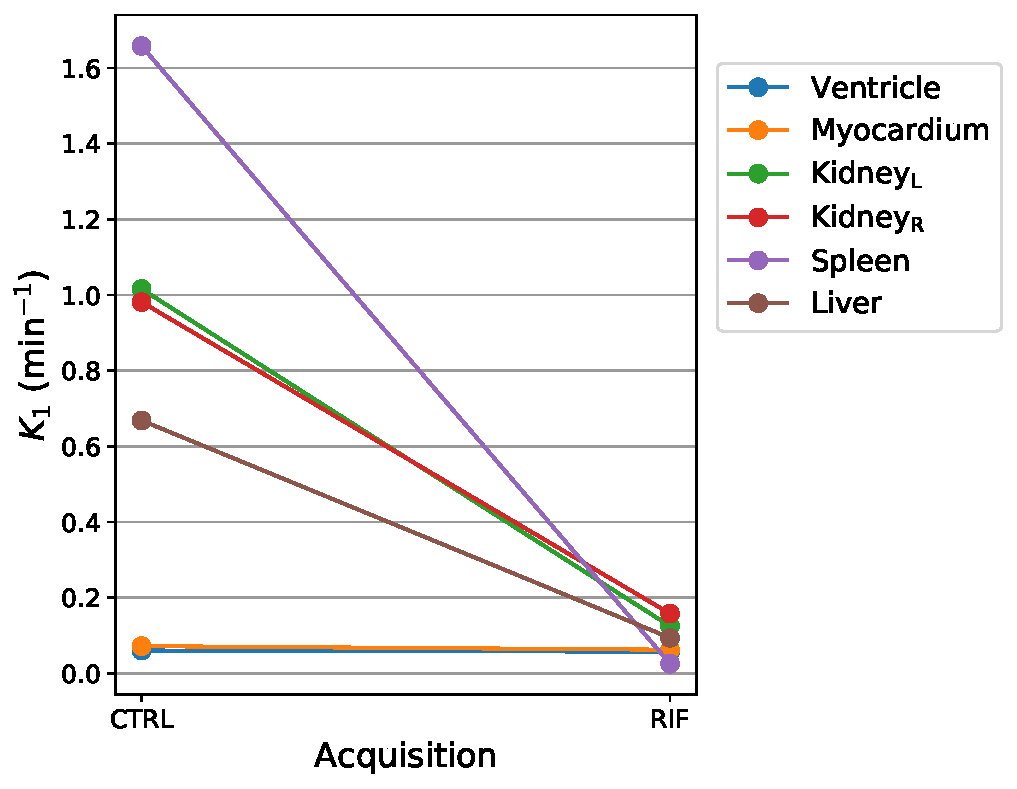
\includegraphics[scale=0.5,angle=0]{3_Results/3_3_DWB_Reconstruction/figures/3_3_IsotoPK_K1_drop.pdf}
\caption{$K_1^{*}$ values as estimated from the 4D spectral reconstruction for VOI regions included in both DSB and DWB acquisitions , shown for the \textit{CTRL} and \textit{RIF} scan}
\label{fig_3_3:IsotoPK_K1_drop}
\end{figure} 

\subsection{Fit errors and residual modelling}
\label{sub_section:residuals}
As seen in figure~\ref{fig_3_3:IsotoPK_CTRL_DWB_4D_vs_3D_Peripheral}, the mismatch of the 3D and 4D spectral reconstruction at the bladder TAC is the strongest from all the evaluated VOIs. The source of this error is the inability of the spectral model to fit the bladder filling process, by any combination of the decaying exponentials convolved with the arterial input function. This mishmash is of particular concern for dynamic reconstruction as it can be the source of errors that propagate spatially during the dynamic reconstruction process over the entire field of view. 
This issue has been addressed in the following work by making use of adaptive residual modeling within the dynamic reconstruction. It was presented during the IEEE/MIC-2020 conference and the following conference record has been submitted for publication. 

\cleardoublepage

%%
%\documentclass[journal]{IEEEtran}


\addto\captionsenglish{\renewcommand{\figurename}{Fig.}}

% correct bad hyphenation here
\hyphenation{op-tical net-works semi-conduc-tor}

%\begin{document}


% paper title
% can use linebreaks \\ within to get better formatting as desired
% Do not put math or special symbols in the title.
\title{\huge Dynamic 4D PET Reconstruction Using the Spectral Model and Adaptive Residual Modelling}

% author names and IEEE memberships
% note positions of commas and nonbreaking spaces ( ~ ) LaTeX will not break
% a structure at a ~ so this keeps an author's name from being broken across
% two lines.
% use \thanks{} to gain access to the first footnote area
% a separate \thanks must be used for each paragraph as LaTeX2e's \thanks
% was not built to handle multiple paragraphs
%
\author{\authorblockN{
Zacharias Chalampalakis, Simon Stute, Marina Filipović, Florent Sureau, Solène Marie, Michel Bottlaender, Nicolas Tournier, and Claude Comtat % <-this % stops a space Bottlaender
}\\
\vspace{0.15cm}
%\authorrefmark{1}Equally contributed\\
%\authorrefmark{1} Imagerie Moleculaire In Vivo, CEA, SHFJ, Inserm, CNRS, Univ. Paris Sud, Univ. Paris Saclay, Orsay, France\\
%\authorrefmark{2} LaTIM, INSERM 1011, CHRU de Brest, France\\  
%\authorrefmark{3}UIMIV U1023 – SHFJ, Orsay, France\\  
%\authorrefmark{4}INCIA, CNRS UMR 5287, Univ. Bordeaux, France\\
%\authorrefmark{5}CRCNA - Centre de Recherche en Cancérologie Nantes-Angers, Nantes, France\\

% The following was added to save space between affiliations and actual text
\vspace{-0.9cm}

\thanks{Manuscript received 15 December, 2020. 
This project has received funding from the European Union's Horizon 2020 research and innovation programme under the Marie Sk\l{}odowska-Curie grant agreement No 764458. This work was performed on a platform of France Life Imaging network partly funded by the grant ANR-11-INBS-0006.

Z. Chalampalakis, M. Filipović, F. Sureau, S. Marie, M. Bottlaender, N. Tournier, and C. Comtat are with Biomaps, Université Paris-Saclay, CEA, CNRS, INSERM, Orsay, France. (e-mail: Zacharias.Chalampalakis@cea.fr). 

S. Stute is with the Nuclear Medicine Department, Nantes University Hospital, CRCINA, INSERM, CNRS, Université d’Angers, Université de Nantes, Nantes, France. } %\protect
\includegraphics[height=0.75em]{eu_flag_yellow.pdf} }
}


% make the title area
\maketitle

\setlength{\abovecaptionskip}{0pt plus 3pt minus 2pt} % Chosen fairly arbitrarily
%-------------------------------------------------------------------------------
%-------------------------------------------------------------------------------
%-------------------------------------------------------------------------------
\begin{abstract}
Application of 4D reconstruction algorithms to dynamic data, especially in whole-body dynamic imaging, can result in spatial propagation of errors over the field of view originating from regions with poor model fits. An adaptive modelling strategy has been previously proposed for this problem to improve the model fit over the field of view, using residual adaptive modelling in the reconstruction process. We used this strategy within a 4D reconstruction algorithm that makes use of the spectral analysis model as a primary model and a PCA based adaptive residual model as a secondary model. The developed algorithm maintains genericity and does not impose strong assumptions about the underlying kinetics. The objective of this work is to evaluate the algorithm on a whole-body dynamic dataset of a healthy volunteer imaged with ${}^{11}$C-Glyburide, a newly developed tracer used in the study of distribution and function of OATP transporters. Results showed improved estimates over the pelvic area where the bladder filling process was poorly fitted by the spectral model alone. The adaptive 4D algorithm has successfully identified and selectively corrected for the filling process, when compared against 3D independent frame reconstructions, while preserving the fit of well-modelled regions. Optimal results were obtained when spatial and temporal filtering of residual data was applied prior to PCA analysis, in which case the adaptive algorithm selectively corrected poorly modelled physiological processes, averted from modelling respiratory motion induced errors and resulted in reduced induction of noise in the reconstruction process.
\end{abstract}

\section{Introduction}
\IEEEPARstart{D}{ynamic} PET has been traditionally utilised in single organ studies, but recently there has been increased interest in whole body dynamic imaging, for research and for potential future clinical applications\cite{Lammertsma2017,Leahy2018,Rahmim2019,Fahrni2019}. Synchronous dynamic PET of the whole body requires scanner geometries that can encompass the entire length of the human body. Although systems capable of whole body axial coverage have been recently developed~\cite{Cherry2017}, their availability is not yet widespread. Current clinical scanners achieve whole body coverage using multiple axial bed positions or acquisition protocols with continuous axial bed motion. Based on these acquisition modes whole body dynamic protocols have been developed that make use of repeated whole body passes~\cite{Karakatsanis2013}. 
Conventional analysis of dynamic data is performed with independent 3D reconstructions of frame data, followed by kinetic model fitting. Whole-body dynamic protocols make the task of reconstruction and subsequent kinetic modelling more challenging due to the introduction of large temporal gaps in the data which can lead to biased estimates and increased noise, especially for parametric maps. 
To improve image quality and account for the noise in the raw data, 4D reconstruction algorithms can be used to directly incorporate the dynamic model of interest in the reconstruction~\cite{Reader2014}.
Depending on the choice of the dynamic model, these reconstructions can directly provide the parameters of interest or temporal regularisation on the reconstruction process of frame data. The spectral analysis model, inspired by the homonym method~\cite{Cunningham1993}, fits on any underlying kinetic behaviour that can be described by compartmental modelling. When used in 4D reconstruction it provides temporal regularisation as well as direct estimation of some kinetic parameters. Use of this model has shown to reduce noise and bias of kinetic parameter estimates when applied on data from whole body dynamic protocols~\cite{Chalampalakis2019}.

When considering the effective field of view of whole body dynamic studies, certain regions might not fulfil the generic assumptions of the spectral analysis model. For example processes such as delay of tracer delivery and non-arterial tracer delivery (ex. bladder filling).
In 4D reconstruction, the tomographic update process is entangled with the dynamic model and errors from the temporal model fit have the potential to spatially propagate to other regions. Due to the fact that raw data from multi-bed whole body dynamic studies are acquired and reconstructed as separate beds, the potential for errors propagation is limited in the bed position where they originate from. It has also been shown that use of time of flight (TOF) information in the reconstruction aids in reducing spatial propagation of errors~\cite{Kotasidis2016a}. Nevertheless, model fit errors have the potential to propagate and when possible should be corrected or accounted for. For this reason, when 4D reconstruction is used and especially when applied on whole body datasets extra consideration has to be given on improving the model fit for all regions.

The application of an adaptive residual model as a second dynamic model has been previously suggested for reducing model fit errors~\cite{Matthews2012}. Its application in 4D reconstruction has been shown to reduce bias at the cost of increased noise for direct estimation of kinetic micro-parameters~\cite{Kotasidis2014c}.
The objective of this work was to implement and evaluate adaptive residual modelling in 4D reconstruction, using real whole body dynamic PET data, with no prior knowledge of the underlying kinetics and the distribution of residuals. For this purpose, the spectral analysis model was used in conjunction with a residual model in 4D reconstruction to maintain genericity in the reconstruction with minimum assumptions on the underlying kinetics. 
The end objective was to assess if adaptive residual modelling can be permanently applied in 4D reconstruction, with no prior knowledge of kinetics and model fit errors, by relying on the selectivity of the algorithm for correction of underlying model fit errors, when and where those arise. 
%-------------------------------------------------------------------------------

\section{Methods}
\subsection{Data acquisition}
Dynamic whole body data using a novel Glyburide (${}^{11}C$-GLB) tracer were acquired from healthy volunteers on a GE Signa PET-MR, using a dedicated dynamic protocol of 5 bed positions to provide sufficient coverage of the body. Glyburide is a substrate of hepatic and extrahepatic Organic Anion Transporting Polypeptides (OATP) which can be isotopically radiolabelled with carbon-11 for PET imaging. The data were acquired as part of the exploratory pharmacokinetic study IsotoPK which is conducted in our centre for studying the distribution of OATP transporters in the body and their role in the delivery of drugs to tissues~\cite{Marie2019}. 
Data from a single volunteer study were used in this work. In detail the dynamic acquisition consisted of a single bed acquisition centred over the liver, imaged for 3 minutes from tracer injection, followed by 14 whole body passes of 9x20s and 5x30s frames for each bed position. 
Arterial blood samples were collected manually during the whole study, to measure the input function.
\subsection{Reconstruction}
The spectral analysis model was used in all 4D reconstructions, using 4 spectral functions with decay rates ranging from 3 \(min^{-1}\) to 0.001 \(min^{-1}\). A constant and a delta function were also included to model tracer trapping and blood fraction. The 4D reconstruction algorithm with adaptive residual modelling was developed using the spectral model as primary model and an adaptive secondary model, similar to the proposed method by Matthews et al.~\cite{Matthews2012}. 
 
The steps of the adaptive residual modelling 4D reconstruction algorithm are:

\begin{enumerate}
  \item Start with image estimate $\lambda_{jf}^{(k)}$, for voxel $j$ and frame $f$ at iteration $k$. 
  \item Perform tomographic update using MLEM to get the EM update image $\lambda_{jf}^{(EM)}$.
  \item Perform primary model fit using the NNLS algorithm on $\lambda_{jf}^{(EM)}$ and estimate model parameters $\bm{\theta}_{j}^{(k+1)}$.
  \item Calculate residuals as $ r_{jf} = \lambda_{jf}^{(EM)} - f_{spectral}(\bm{\theta}_{j}^{(k+1)}) $.
  \item Perform PCA analysis on residuals to estimate a set of residual basis functions (RBF) which form the secondary (adaptive) model. 
  \item Estimate modelled residuals $g_{jf}$ from the LS fit of the secondary model on the $r_{jf}$ data. 
  \item Estimate optimal fraction $K_{j}$ for residuals re-introduction, using generalised cross validation.
  \item Add fraction of modelled residuals in image estimate $\lambda_{jf}^{(k+1)} = f_{spectral}(\bm{\theta}_{j}^{(k+1)}) + K_{j} g_{jf} $ and repeat from step 2.
\end{enumerate}

where NNLS stands for Non-Negative Least Squares and $f_{spectral}$ is the spectral model which provides activity distribution maps for all frames, given model parameters $\bm{\theta}_{j}$. 
        
In step (5) of our adaptive modelling implementation, the residual data were spatially smoothed with an isotropic Gaussian kernel of 32mm FWHM, to enhance the PCA analysis results. Smoothing of the residuals was not however applied in the fitting process of the secondary model in step (6). A fixed number of the most significant PCA components was used as basis functions of the adaptive residual model. The components were updated on each iteration of the 4D algorithm.

For the estimation of the optimal fraction $K_{j}$, the following equation from Matthews \textit{et al.}~\cite{Matthews2012} was used, which is derived from generalised cross-validation,

\begin{equation}
K_{j} = \frac{1-\frac{r_{df}}{r_{RSS}}}{1-r_{df}} , 
\end{equation}

where $r_{df} = \frac{n_s}{n_f - n_p}$, with $n_p$ and $n_s$ being the number of parameters of the primary and secondary model respectively, and $r_{RSS}$ being the fraction of modelled to measured residuals sum of squares. 

% with the $r_{df}$ ratio of degrees of freedom of the residual model to residual space being  0.375(0.25).

The dynamic data from each bed of the study were reconstructed as individual frames using 3D MLEM (150it), using 4D reconstruction (300it) and with the developed adaptive algorithm 4D-ResidMod (300it). The adaptive reconstruction algorithm was evaluated using the 2 and 3 most significant PCA components as RBFs, referred to as 4D-ResidMod-2RBF and 4D-ResidMod-3RBF respectively. We also implemented a version of the adaptive algorithm with the addition of temporal Gaussian smoothing of 62s FWHM applied on the residual data used for PCA analysis in step (5) of the algorithm, referred as reconstruction 4D-ResidMod-3RBF-Tempfilt.

All reconstructions were performed with the open source reconstruction platform CASToR~\cite{Merlin2018}, using PSF modelling and TOF information. Correction for motion has not been included in the reconstructions. PCA analysis was performed using the Eigen library~\cite{eigenweb}. 
%------------------------------------------------------------------------------

\section{Results}
As seen in Fig.~\ref{fig:Frame14Differences} (top row) by the difference in activity estimates from 3D and 4D reconstruction in a late frame, the 4D algorithm with the spectral model alone resulted in lower activity estimates over the bladder region and higher activity estimates in some large blood vessels at the shoulders and pelvic regions. No noticeable differences were seen in other areas, apart from random variations in activity due to differences in noise levels of the compared reconstructions.
As expected, the filling process of the bladder seen in the bladder time activity curve from 3D reconstruction in Fig.~\ref{fig:TACs} (bottom row) cannot be modelled by the spectral model because the filling process is not directly relatable to arterial tracer delivery at the local (voxel) level. Differences in some large blood vessels could potentially be attributed to delay of the input function, which is not accounted for in the spectral model where a single input function is assumed to apply for all regions. 

Reconstruction of the data with adaptive residual modelling resulted in improved estimation of the bladder filling process, for both options of residual modelling using 2 and 3 residual basis, as it can be seen in the difference images of Fig.~\ref{fig:Frame14Differences} (middle row) and the bladder TAC in Fig.~\ref{fig:TACs}. 
No improvements were seen for the differences at the blood vessels of the shoulders and pelvic regions. 

At the liver, where most of the tracer uptake is concentrated, 4D and 3D reconstruction TACs show a subtle mismatch between 1100 and 1500 seconds (Fig.~\ref{fig:TACs}, top row). Analysis on the liver dome VOI (Fig.~\ref{fig:TACsFilt}, top row) clearly shows this difference, which originates from underlying respiratory motion that has been captured in the PET dynamic data. 4D reconstruction alone was unable to model these fluctuations, as expected, but the adaptive algorithm using 3 residual basis has achieved to model for this behaviour as seen in Fig.~\ref{fig:TACsFilt}.
Since physiological kinetic processes, whether sufficiently modelled or not, are not expected to result in sudden changes of activity between adjacent frames, we implemented a version of the algorithm with temporal smoothing prior to PCA analysis to prevent from modelling changes due to fast processes such as respiratory motion. On this case this algorithm (4D-ResidMod-3RBF-Tempfilt) has managed to maintain the selective adaptive modelling behaviour over the bladder while avoiding fitting the motion related effects over the liver dome as seen in Fig.~\ref{fig:TACsFilt}. 

\begin{figure} [h!]
\centering
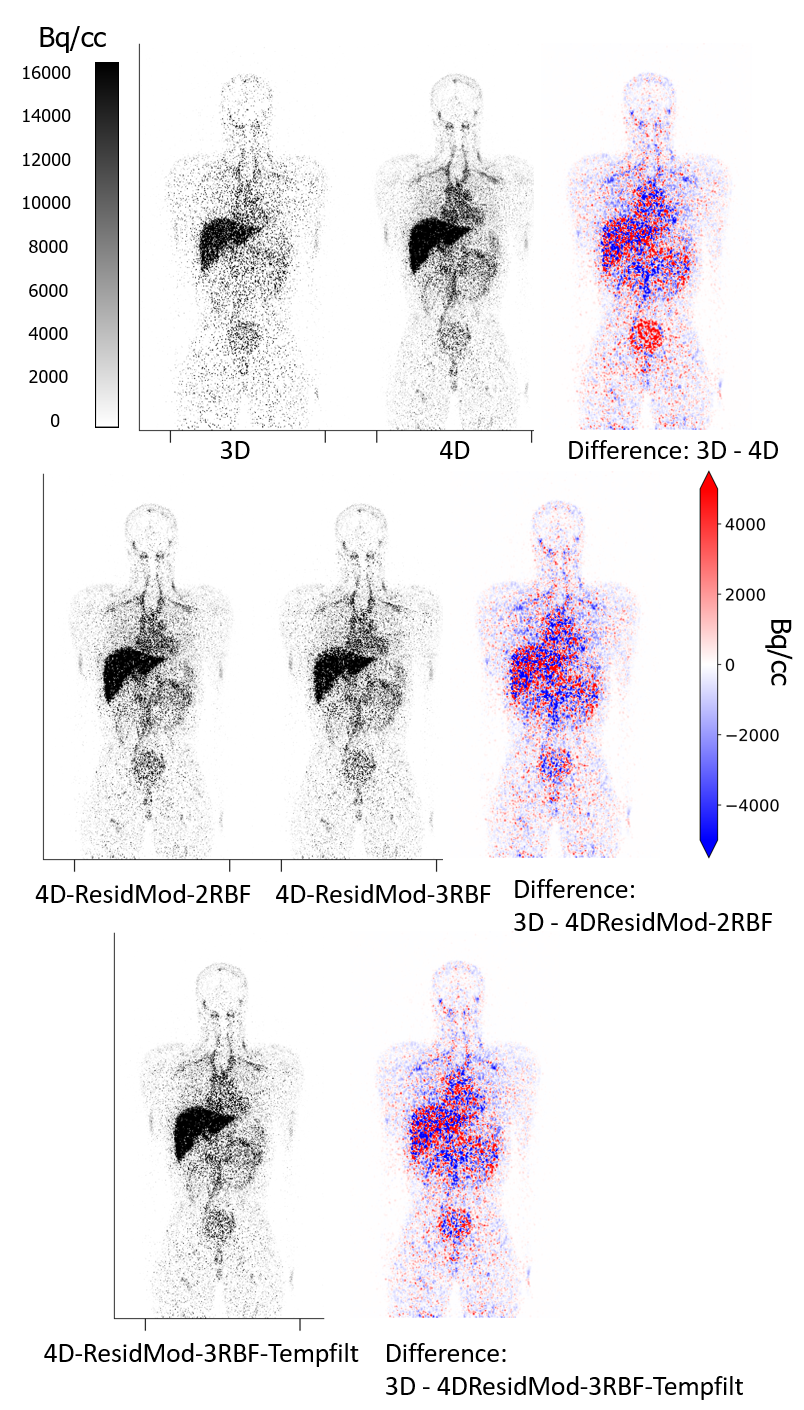
\includegraphics[scale=1.1, angle=0]{3_Results/3_3_DWB_Reconstruction/MIC2020/Frame14DifferencesV2.png}

\caption{Coronal view of activity distribution from the evaluated reconstructions (frames of 41.2 to 44.1 minutes post injection). Difference images are also shown for selected cases against the 3D reconstruction.}
\label{fig:Frame14Differences}
\end{figure}

\begin{figure} [h!]
\centering
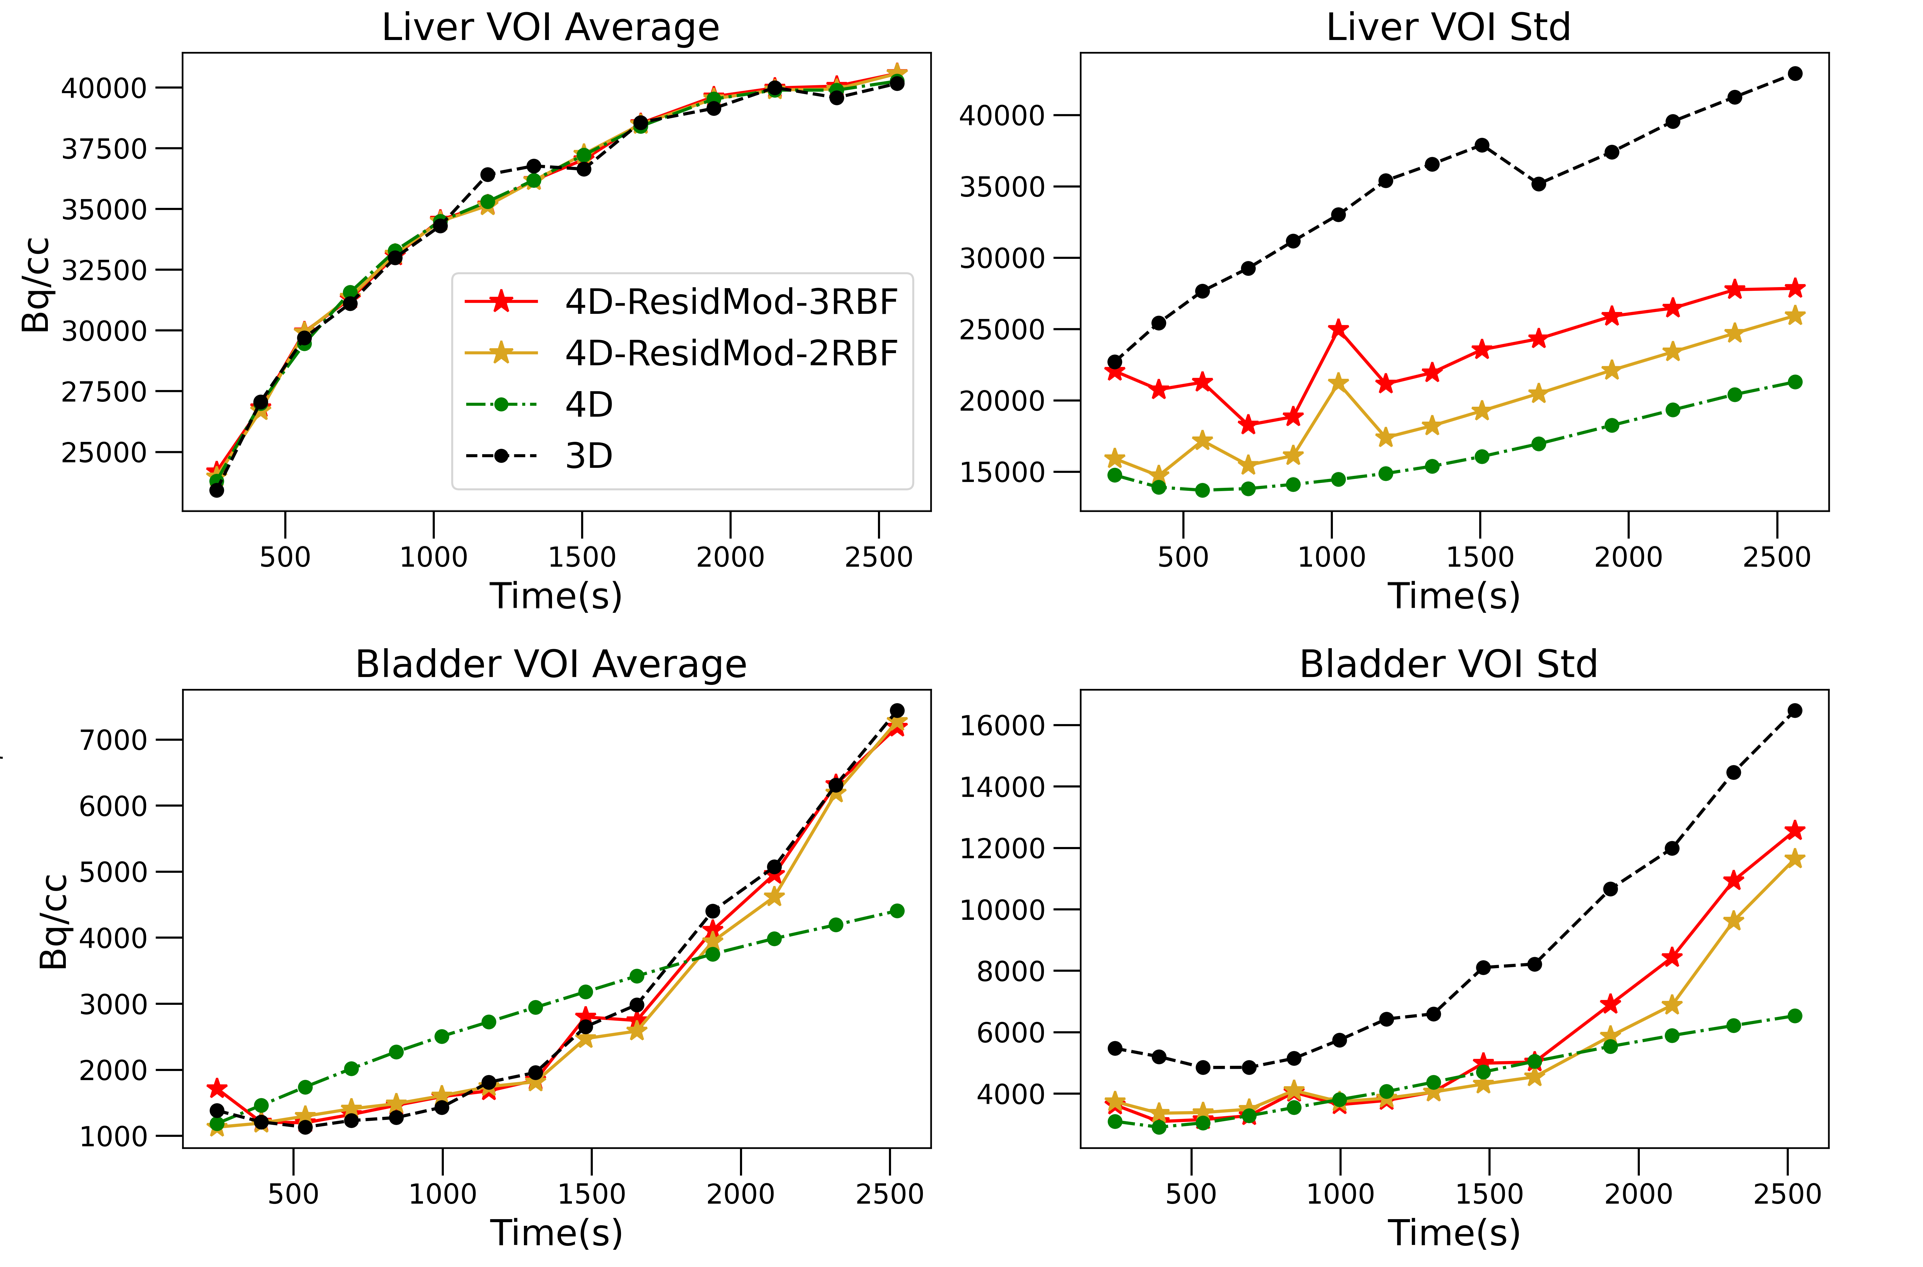
\includegraphics[scale=0.44,angle=0]{3_Results/3_3_DWB_Reconstruction/MIC2020/TACs.png}
\caption{Average and standard deviation time curves of the liver and bladder VOIs, for the comparison of 3D to 4D reconstruction results as well as 4D reconstruction with residual modeling using different number of residual basis functions.} 
\label{fig:TACs}
\end{figure}

\begin{figure} [h!]
\centering
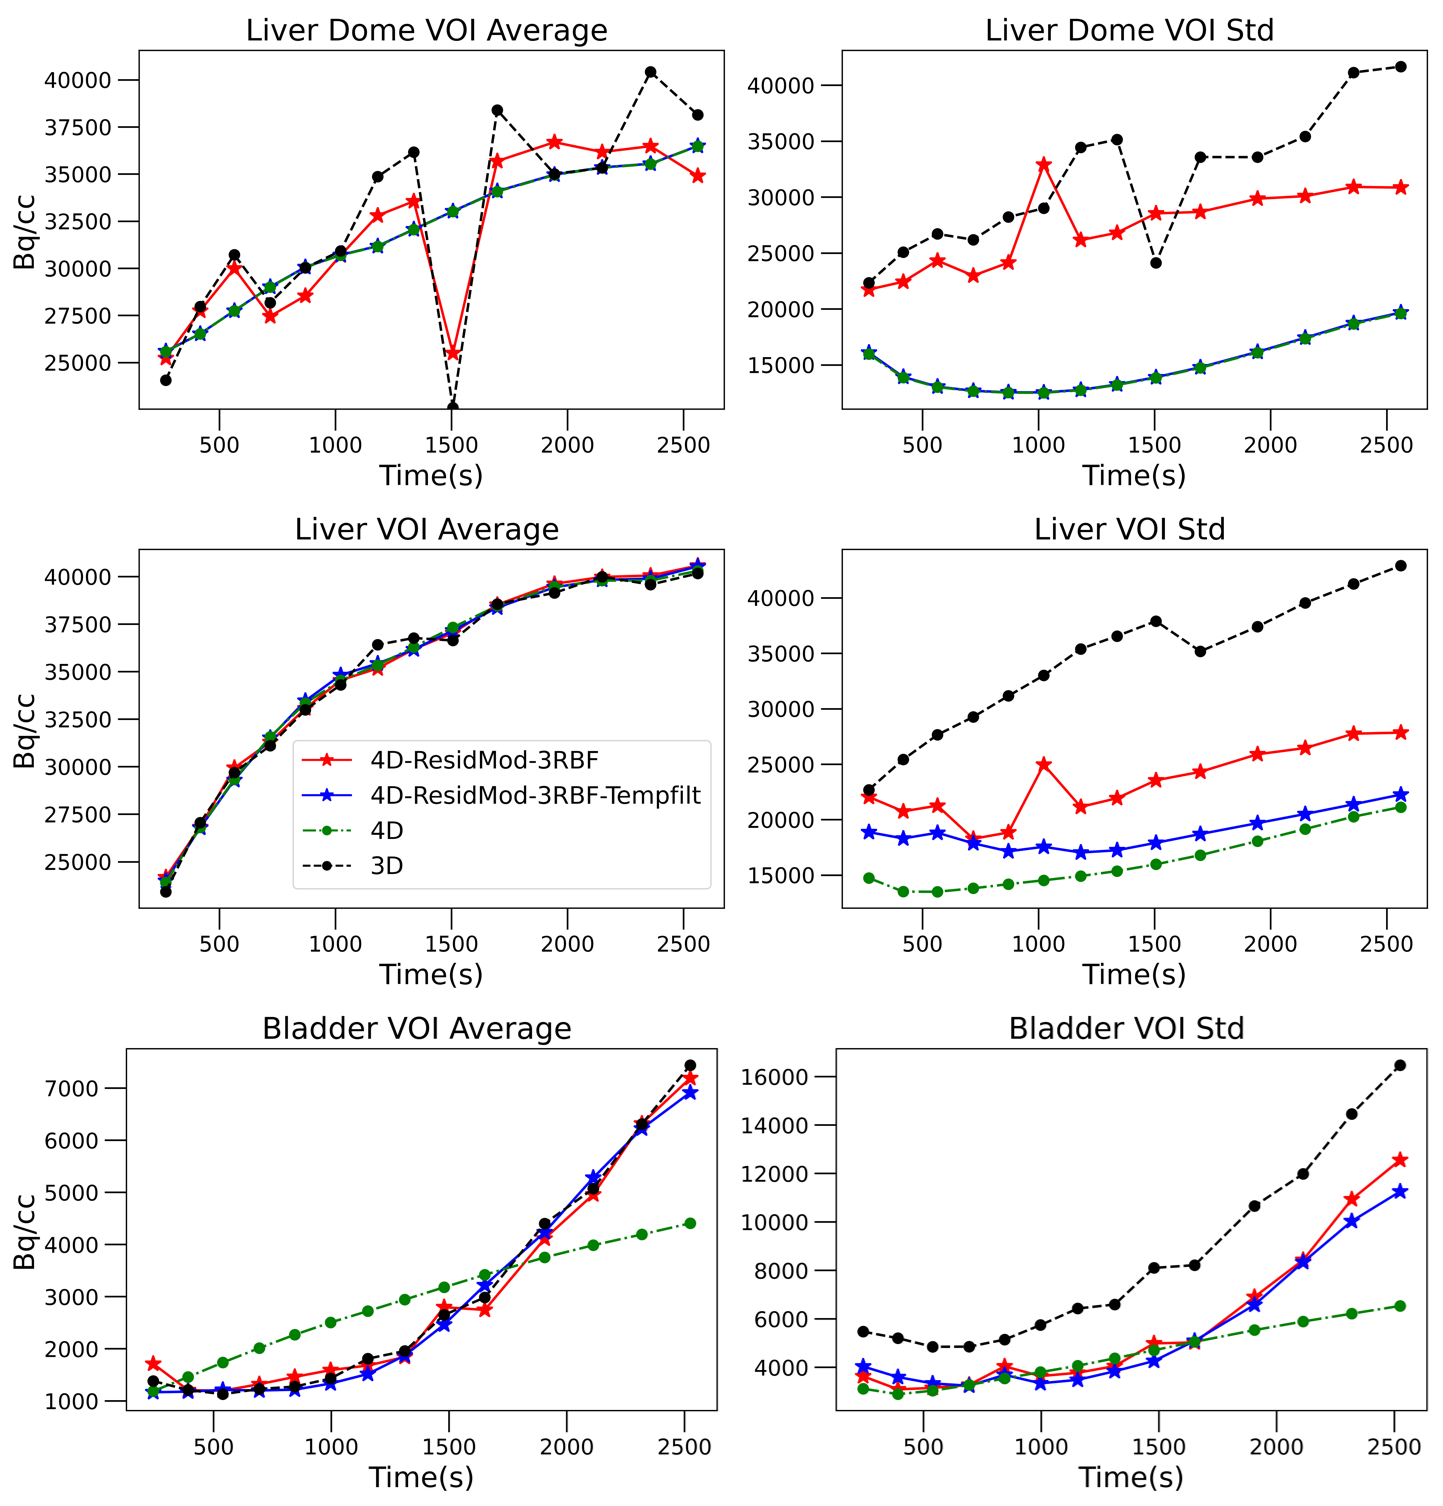
\includegraphics[scale=0.58 ,angle=0]{3_Results/3_3_DWB_Reconstruction/MIC2020/TACsFilt.png}
\caption{Average and standard deviation time curves of the dome of the liver the whole liver and bladder VOIs, for the comparison of 4D reconstruction with residual modeling with and without temporal filtering of residuals.} 
\label{fig:TACsFilt}
\end{figure}


In all regions of the effective FOV the addition of adaptive modelling has resulted in the increase of image noise, compared to 4D reconstruction, with the higher number of residual basis resulting in higher noise. The introduction of temporal filtering in the adaptive model estimation process has aided in reducing the induction of noise for the majority of the evaluated regions in our study. 
A comparison of the effect on image noise across regions within this whole body study can be made by the VOIs standard deviation shown in Fig.~\ref{fig:BarPlot} for all evaluated algorithms.
An example map of the fraction $K_{j}$ and the modelled residuals $g_{jf}$ is given in Fig.~\ref{fig:FractionMap}. These maps demonstrate the desired selectivity of the algorithm, concentrated over the bladder in this case, but also the
spill of noise from the residual space in these maps which is subsequently added in the reconstruction process.

\begin{figure} [h!]
\centering
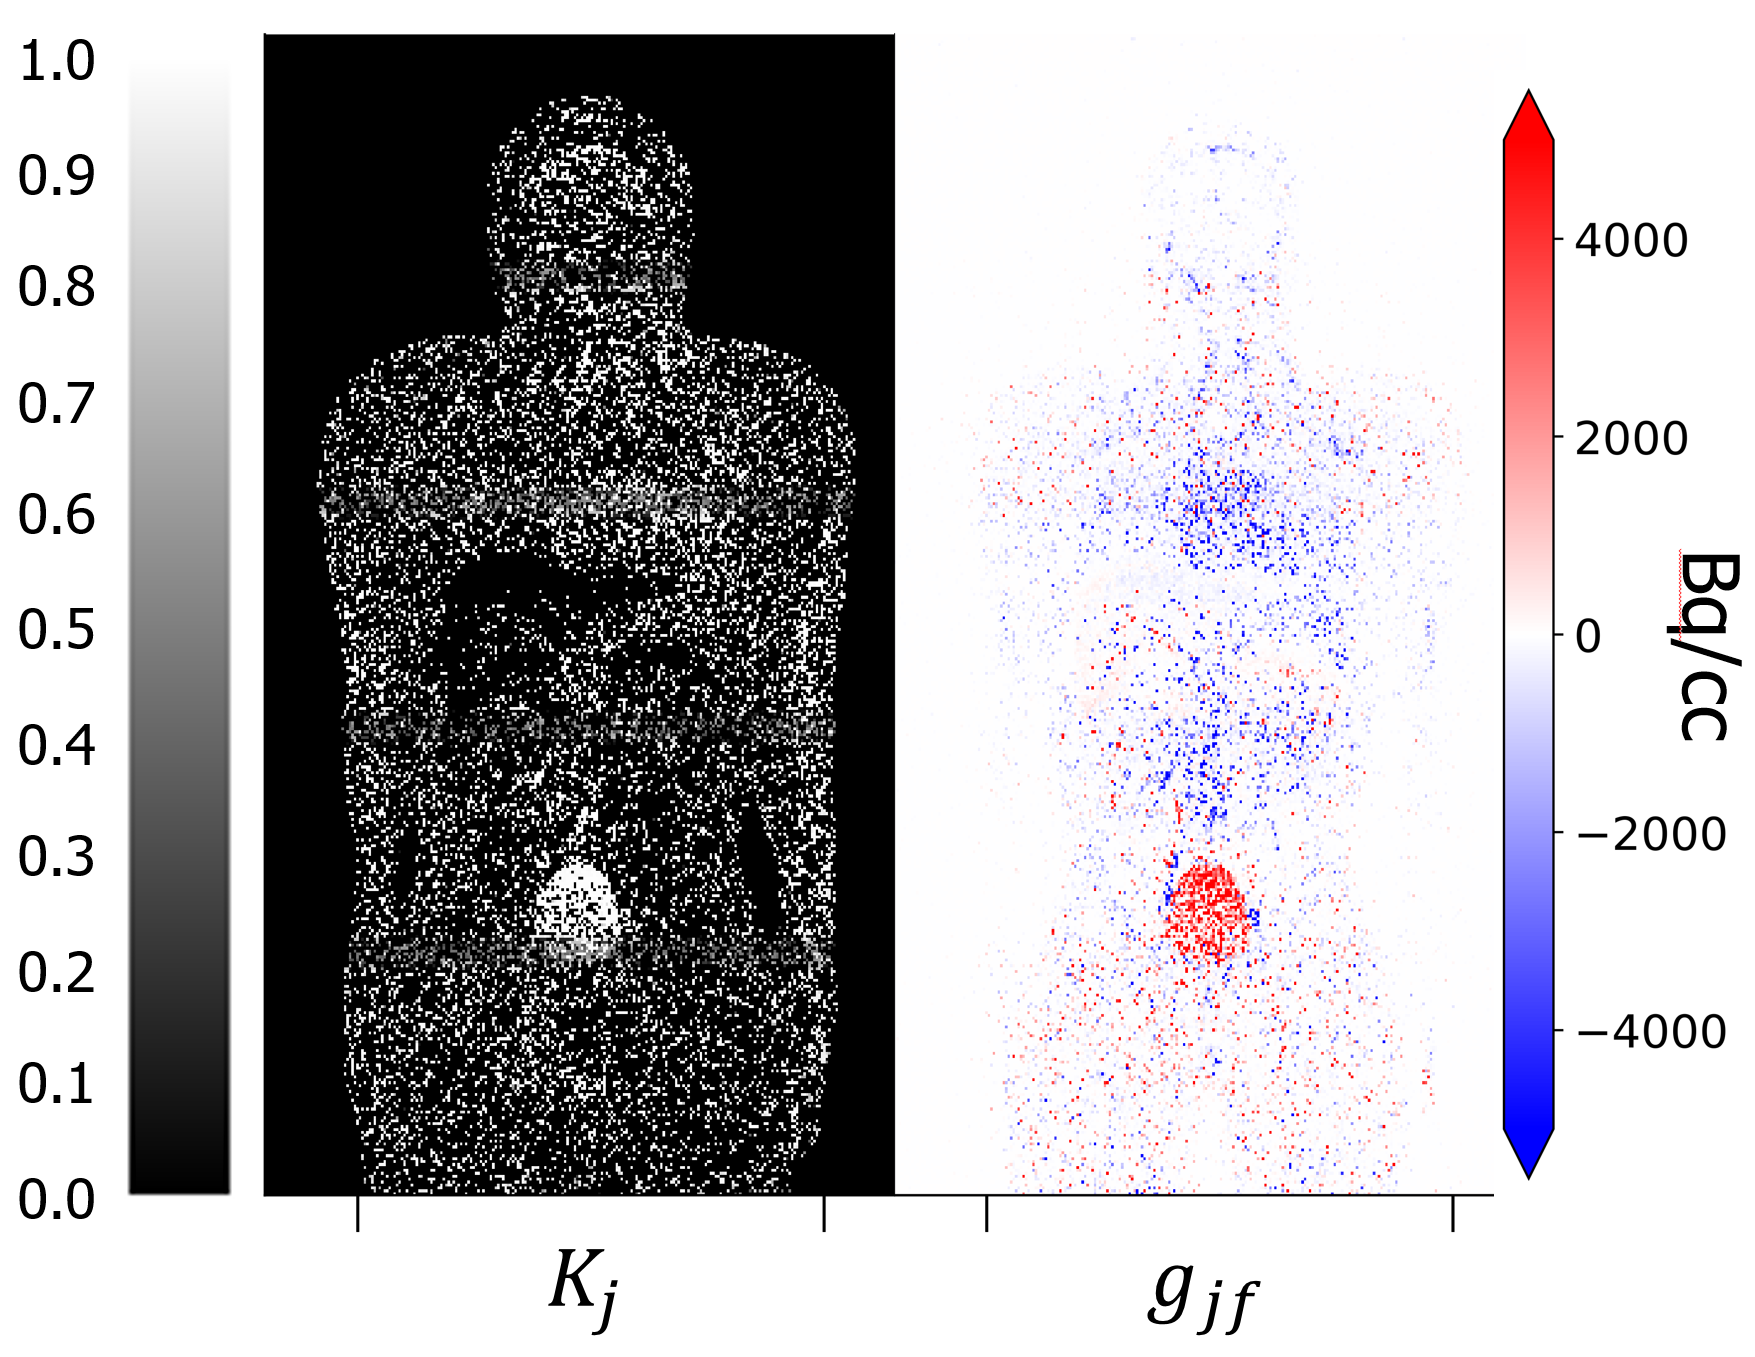
\includegraphics[scale=0.44 ,angle=0]{3_Results/3_3_DWB_Reconstruction/MIC2020/FractionMap.png}
\caption{Fraction map of $K_j$ and modelled residuals $g_{jf}$ of the residual model 4D-ResidMod-3RBF-Tempfilt at iteration 75.} 
\label{fig:FractionMap}
\end{figure}

\begin{figure} [h!]
\centering
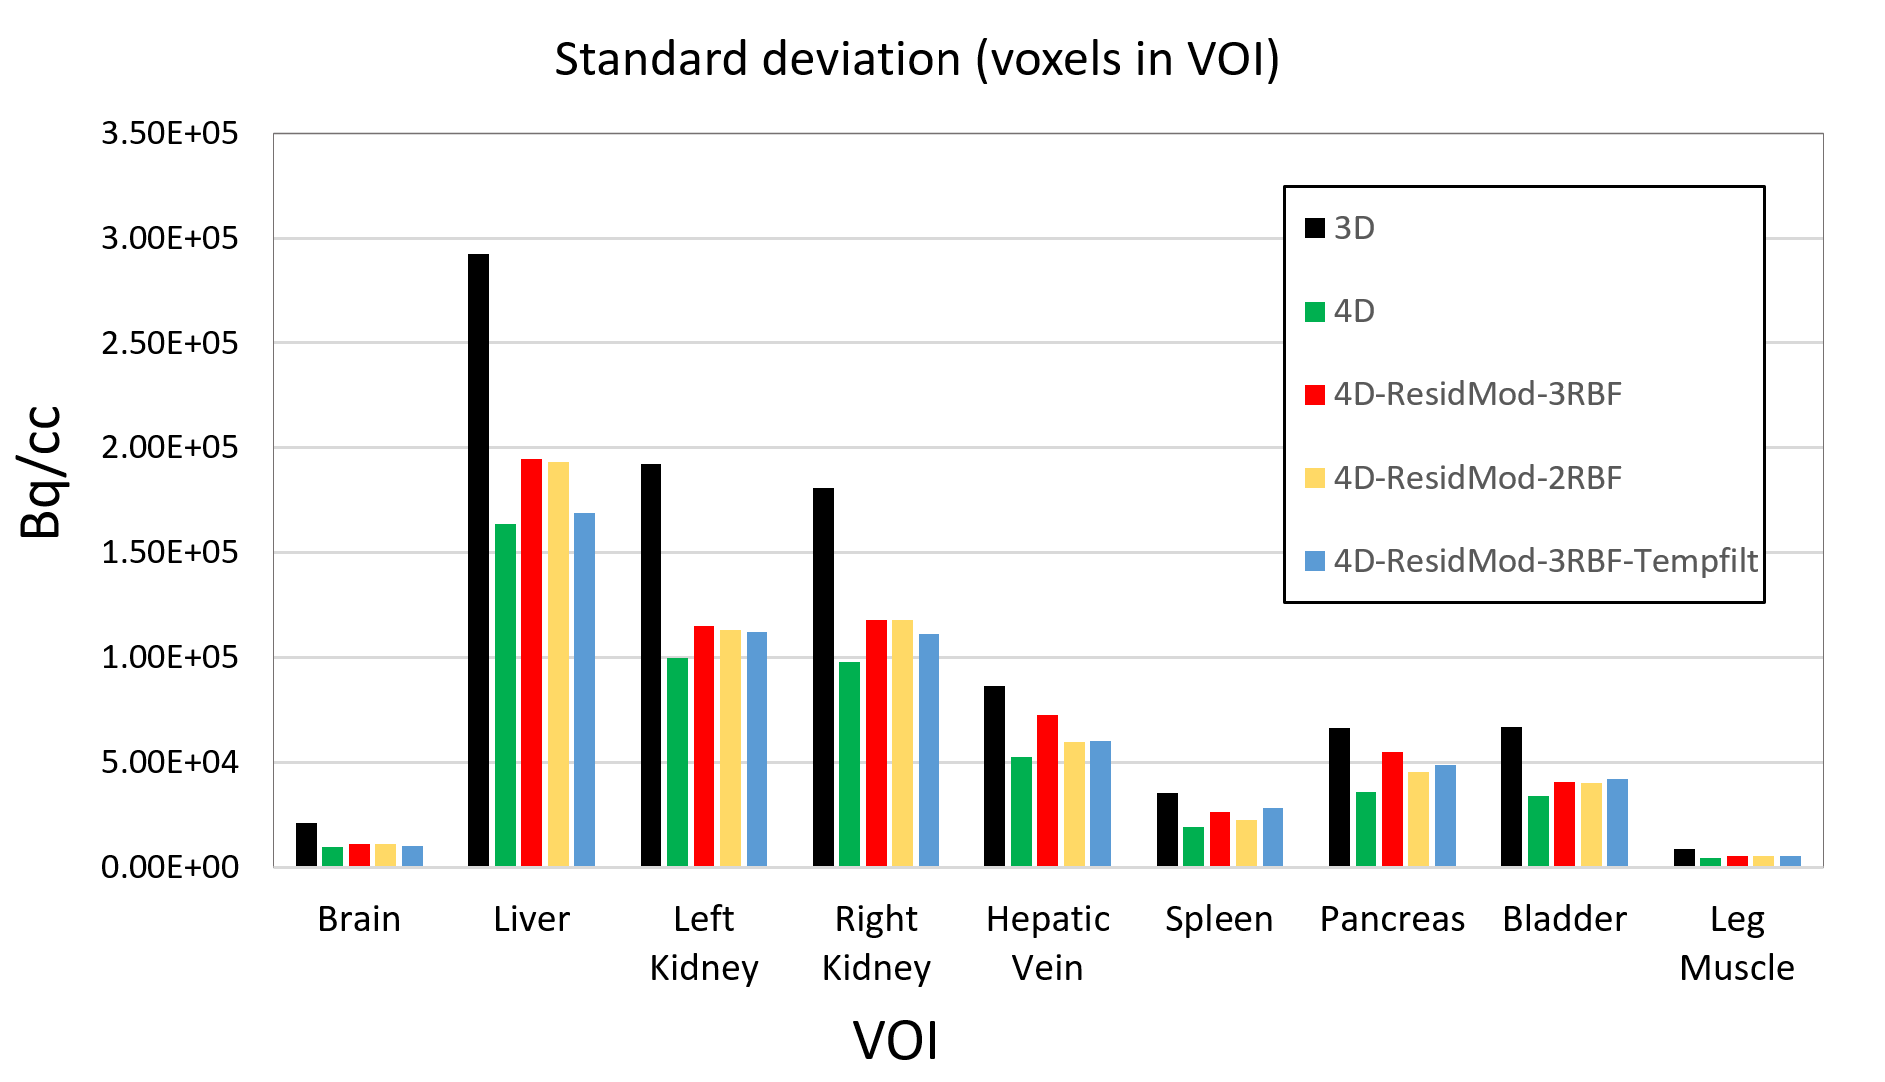
\includegraphics[scale=0.45 ,angle=0]{3_Results/3_3_DWB_Reconstruction/MIC2020/BarPlot.png}
\caption{Standard deviation of VOIs for regions in the whole-body, for all evaluated reconstructions.} 
\label{fig:BarPlot}
\end{figure}


\section{Discussion and Conclusion}
General dynamic models such as the spectral analysis model can be useful in 4D reconstruction of whole body dynamic data using new tracers, as they do not impose strong assumptions about the underlying kinetics. But over the effective field of view of whole body dynamic studies certain regions and their physiological processes might not fulfil the general assumptions of the model. In these cases, the adaptive residual modelling strategy can be utilised to improve parameter estimates for these regions and help in minimising the risk of spatial propagation of errors to other well modelled regions.

%Due to the fact that raw data from multi-bed whole body dynamic studies are acquired and reconstructed as separate beds, the potential for errors propagation is limited in the bed position where they originate from. Also it has been shown that use of time of flight (TOF) information in the reconstruction aids in reducing spatial propagation of errors~\cite{Kotasidis2016a}. Nevertheless model fit errors have the potential to propagate and when possible should be corrected or accounted for.

In this work, 4D reconstruction with the spectral analysis model and adaptive residual modelling was applied on real whole body dynamic data from a first in man study of a new tracer. The algorithm identified and selectively corrected the image activity estimates over the poorly modelled bladder region, by modelling the residuals of that region. This resulted in a 4D reconstruction that did not suffer from the model fit errors over the bladder and potential errors propagated to other regions originating from the bladder region. 
The use of the adaptive model as a secondary model increased the complexity of the modelling in the reconstruction process and resulted in an increase of image noise, with higher number of residual basis functions resulting in higher image noise as expected and inline with previous observations in a simulation study~\cite{Kotasidis2014c}.
In our work we saw that noise from the residual space propagates in the modelled residuals and the optimum fraction values of the secondary model, seen in Fig.~\ref{fig:FractionMap}, and is subsequently re-introduced in the reconstruction process. 

Motion will unavoidably always be present in the raw data of dynamic studies and when it is not accounted for in the 4D reconstruction process will give rise to model fit errors. In our evaluation we saw that the adaptive algorithm attempted to model residuals caused by respiratory motion, when the level of complexity of the secondary model permitted that, even though this was not its original intended use.
As any tracer's kinetic processes are expected to be slower than variations due to respiratory motion, pre-treatment of residuals with temporal filtering in the residual model estimation step aided in averting the adaptive model from fitting these motion induced differences while maintaining its capability of modelling kinetic processes. In addition, temporal filtering also aided in reducing the increase in noise from the use of the secondary model.

In this work we conclude that the use of the secondary adaptive model based on PCA analysis can be a practical solution to spectral analysis model fit errors, when added to the generic 4D reconstruction algorithm used with whole body dynamic data from new tracers. The combination of spatial and temporal filtering in the treatment of residual data prior to PCA analysis provided the optimal results in our tests, in terms of algorithm selectivity and levels of added noise. 


%Finally it is expected that the behaviour of the adaptive model will strongly be affected by the nature of the underlying kinetics and the raw data, so the option of its parameters (number of basis, strength of spacial and temporal filtering, iterations of the model) will need to be fine tuned for each study. 


%\begin{thebibliography}{10}
\bibliography{refs} 
\bibliographystyle{ieeetr}
%\scriptsize

%\bibitem{Reader2014}
%Reader \textit{et al}.
%\newblock Phys. Med. Biol., vol. 59, pp. R371-R418, 2014.
%\bibitem{Chalampalakis2019}
%Chalampalakis \textit{et al}.
%\newblock 2019 IEEE NSS/MIC, Manchester, UK, 2019, pp. 1-3.
%\bibitem{Matthews2012}
%Matthews \textit{et al}.
%\newblock 2012 IEEE NSS/MIC, Anaheim CA, USA, 2012, pp. 3925-3929.
%\bibitem{Kotasidis2014}
%Kotasidis \textit{et al}.
%\newblock Phys. Med. Biol., vol. 59, pp. 6061-6084, 2014.
%\bibitem{Tournier2013}
%Tournier \textit{et al}.
%\newblock AAPS J., vol.15, pp. 1082‐1090, 2013.
%\bibitem{Merlin2018}
%Merlin \textit{et al}.
%\newblock Phys. Med. Biol., vol. 63, pp. 185005, 2018.


% -------------------------------------------------------------
%\bibitem{Rahmim2019}
%Rahmim \textit{et al}.
%\newblock Dynamic whole-body PET imaging: principles, potentials and applications. European Journal of Nuclear Medicine and Molecular Imaging, vol. 46, pp. 501-518, 2019.
% -------------------------------------------------------------
%\bibitem{Karakatsanis2013}
%Karakatsanis \textit{et al}.
%\newblock Dynamic whole-body PET parametric imaging: I. Concept, acquisition protocol optimization and clinical application. Phys. Med. Biol., vol. 58, pp. 7391-7418, 2013.
% -------------------------------------------------------------
%\bibitem{Cherry2017}
%Cherry \textit{et al}.
%\newblock Total-Body PET: Maximizing Sensitivity to Create New Opportunities for Clinical Research and Patient Care. Journal of Nuclear Medicine 2018. vol. 59, pp. 3–12.
% -------------------------------------------------------------
% \bibitem{Reader2014}
% Reader \textit{et al}.
% \newblock 4D image reconstruction for emission tomography. Phys. Med. Biol., vol. 59, pp. R371-R418, 2014.
% -------------------------------------------------------------
%\bibitem{Reader2007}
%Reader \textit{et al}.
%\newblock Fully 4D image reconstruction by estimation of an input function and spectral coefficients. IEEE Nuclear Science Symposium Conference Record, vol. 5, pp. 3260-3267, 2007.
% -------------------------------------------------------------
% \bibitem{Chalampalakis2019}
% Chalampalakis \textit{et al}.
% \newblock Whole-Body dynamic PET: Effect of temporal gaps on FDG Ki quantification from 3D and 4D reconstruction algorithms.2019 IEEE Nuclear Science Symposium and Medical Imaging Conference (NSS/MIC), Manchester, United Kingdom, 2019, pp. 1-3.
% % -------------------------------------------------------------
% \bibitem{Matthews2012}
% Matthews \textit{et al}.
% \newblock Adaptive parametric kinetic modelling for improved full field of view fitting of PET data. 2012 IEEE Nuclear Science Symposium and Medical Imaging Conference Record (NSS/MIC), Anaheim, CA, 2012, pp. 3925-3929.
% % -------------------------------------------------------------
% \bibitem{Kotasidis2014}
% Kotasidis \textit{et al}.
% \newblock Application of adaptive kinetic modelling for bias propagation reduction in direct 4D image reconstruction. Phys. Med. Biol., vol. 59, pp. 6061-6084, 2014.
% % -------------------------------------------------------------
% \bibitem{Tournier2013}
% Tournier \textit{et al}.
% \newblock Effects of selected OATP and/or ABC transporter inhibitors on the brain and whole-body distribution of glyburide. AAPS J., vol.15, pp. 1082‐1090, 2013.
% % -------------------------------------------------------------
% \bibitem{Merlin2018}
% Merlin \textit{et al}.
% \newblock CASToR: A generic data organization and processing code framework for multi-modal and multi-dimensional tomographic reconstruction. Phys. Med. Biol., vol. 63, pp. 185005, 2018.
% -------------------------------------------------------------

%\end{thebibliography}

% that's all folks
%\end{document}

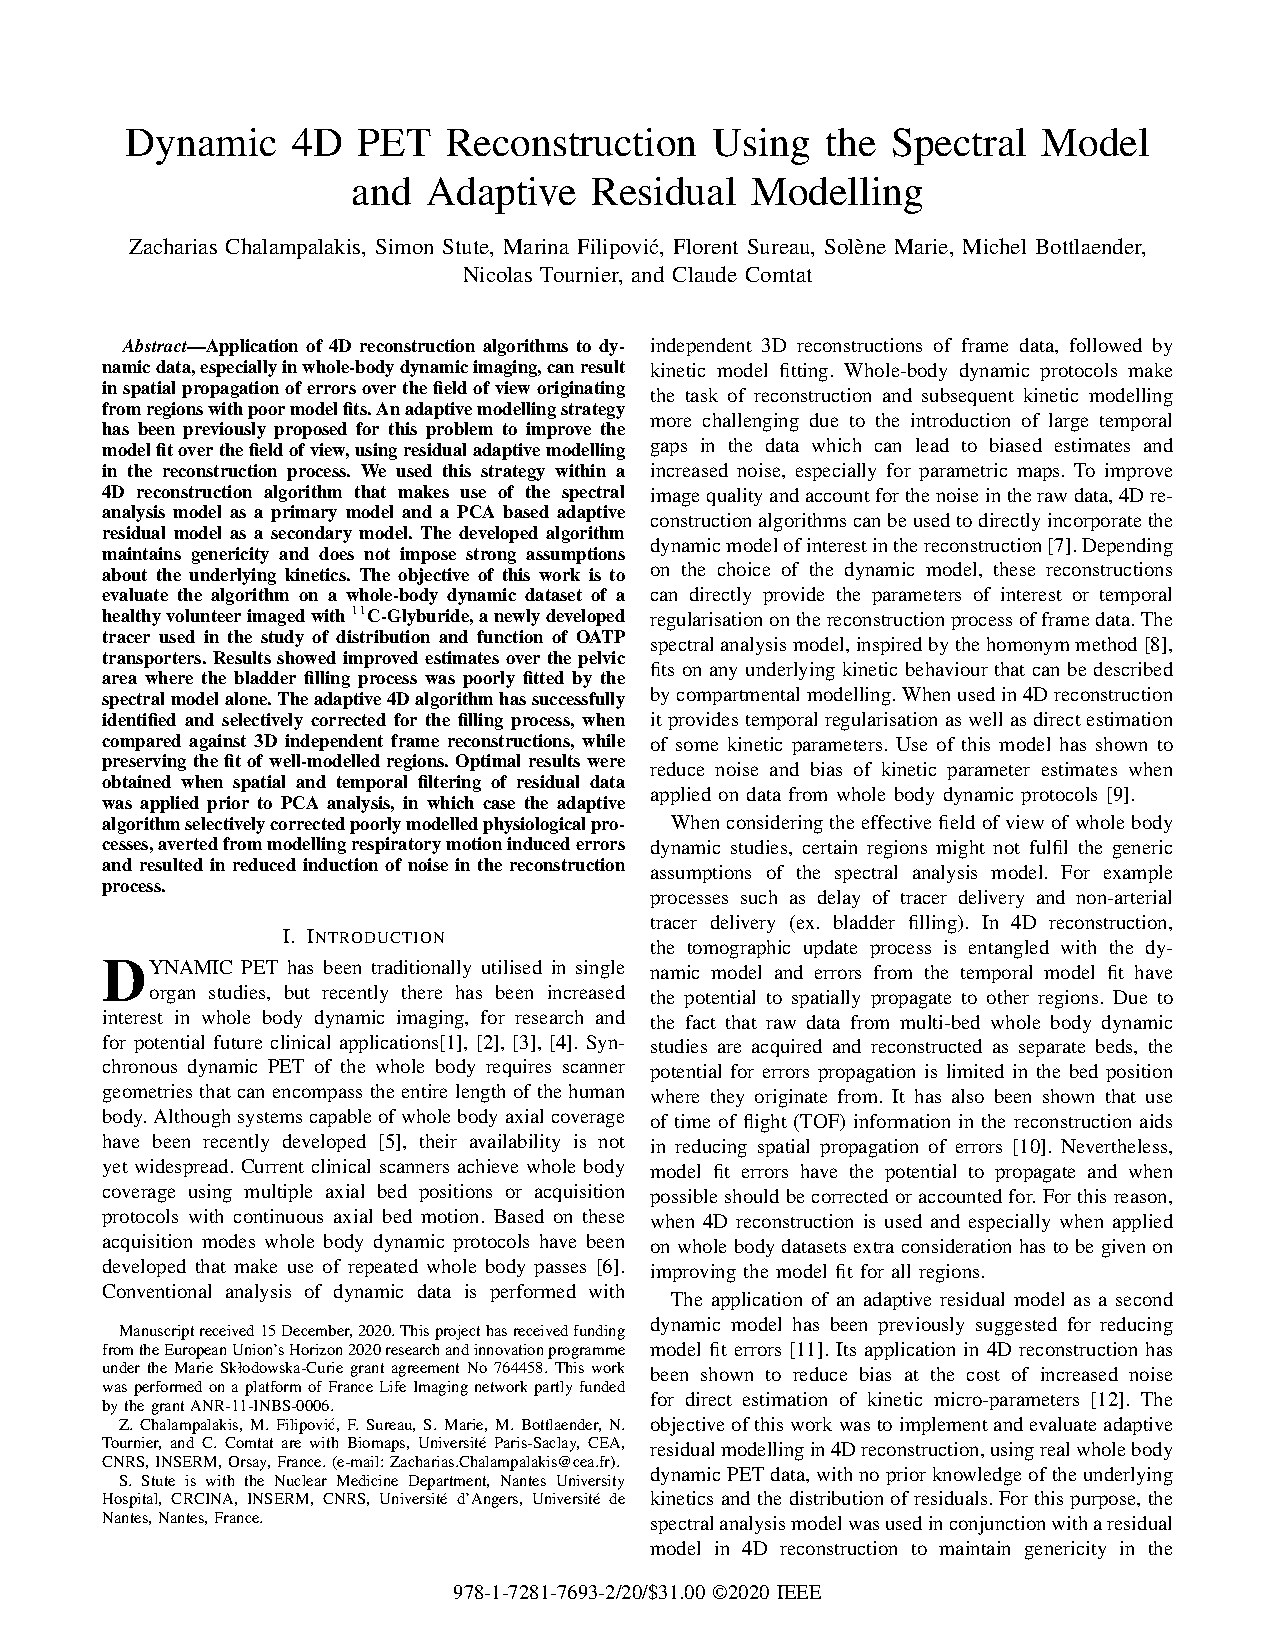
\includepdf[pages=-,pagecommand={}]{3_Results/3_3_DWB_Reconstruction/MIC2020/Whole_Body_dynamic_PET_direct_4D_reconstruction_with_adaptive_modelling__Conference_Record_.pdf}

\section{Discussion}

We have developed and presented a framework for direct multi-bed dynamic reconstruction of DWB data, that allows for synchronous use of both DSB and DWB data that are typically acquired for dynamic studies over the whole body~\cite{Karakatsanis2013}. 
This framework can be used for dynamic reconstruction by making use of the accurate positional and timing information of all the individual bed raw PET data within a single iterative loop, performed either directly within a single system matrix or using the nested optimization approach.
In this study we have tested this framework with real DWB data, from a first in man pharmacokinetic study, where the spectral model was used within the reconstruction to avoid having to assume and enforce a specific compartmental model.
The result (temporally regularised) activity images show estimates with smooth transition in the axial direction across the effective FOV, in terms of image activity values and image noise. Although we hypothesised that use of the data within a single iterative loop results in improved estimates over the overlap region, compared to state of the art methods that perform parametric image overlapping  after reconstruction~\cite{Karakatsanis2016a,Hu2020}, we do not directly compare with these methods. To address this comparison, we performed an evaluation study for these methods using the NHP dataset of chapter~\ref{Chap3_1:AcquisitionOptimization}, but results were inconclusive and showed the need for a detailed simulation study to assess differences in terms of bias and noise properties of the overlapping regions against known ground truth simulated values. 

The IsotoPK real DWB data used in this study included a 180 s DSB acquisition centred over the liver prior to the DWB acquisition. This has enabled the estimation of $K_1^{*}$ parametric images over the region covered by both DSB and DWB acquisitions. As shown before in chapter~\ref{Chap3_2:SimStudy}, that initial information is crucial for estimation of $K_1$. Thus, although use of the DSB initial phase allows for adequate sampling of fast kinetics and estimation of fast kinetics sensitive parameters in DWB studies, it still limits the estimation for parametric images to an axial coverage of a single bed position. All other regions outside this bed coverage were sampled with an 180 s delay, which as shown in chapter~\ref{Chap3_2:SimStudy} produces erroneous estimates of $K_1^{*}$. 
In this study this relates to $K_1^{*}$ estimates in regions outside the coverage of the DSB acquisition in figure~\ref{fig_3_3:IsotoPK_K1_MIP} and figure~\ref{fig_3_3:IsotoPK_K1_SingleSlice}. 
Further investigation in the setup of the acquisition protocol is required to quantify the minimum amount of fast kinetics sampling required for reliable deduction of parametric $K_1$ images and other parametric images sensitive to early fast kinetics. An analogous study conducted for the estimation of 2TC micro-parameters in FDG imaging resulted in evaluation of sensitivity of micro-parameters against sampling of specific time points~\cite{Zuo2019}. A similar study for the spectral model analysis method can evaluate the need of the DSB phase for estimation of $K_1$ and other parameters and if possible adapt the acquisition for reliable estimation of those parameters over the whole effective FOV. 
Another disadvantage of the need for an DSB acquisition is the uneven sampling over different locations of the effective FOV that results to different noise properties across the axial direction. Equal sampling of all regions is proffered to provide comparable noise properties in the axial direction of the FOV.

There are many challenges and limitations in dynamic reconstruction and parametric imaging, which are of particular concern for DWB imaging where the dynamic model is applied over the whole body~\cite{Gallezot2019}. 
Firstly, a single input function has been used for the estimation of the basis functions of the spectral model which is then applied over the entire effective FOV. The use of a single input function does not account for dispersion and delay effects that are varying for different location in the body. As kinetic models and in particular the spectral model rely heavily on the input function, any errors or inaccuracies can lead to considerable estimation errors. Ideally the delay and dispersion properties of the input function need to be estimated for each region, which would then be used for calculating a set of spatially variant spectral basis functions.
Furthermore, the input function was derived from manual samples whose sampling frequency compromises the measurements of the peak of the input function. This information over the peak is of significant importance for estimation of micro-parameters. 
Methods for joint-estimation of dispersion and delays or joint estimation of the input function itself within the reconstruction process have been previously proposed~\cite{Wang2013,Reader2014}, but so far have only been applied in DSB studies~\cite{Reader2014} and studies using total-body data~\cite{Feng2019} where sensitivity and sampling-frequency are much higher compared to multi-bed DWB imaging.
Many considerations are needed to evaluate translation of these methods in multi-bed DWB, where the poorer data statistics and sampling frequency might not allow for reliable estimation of all the involved parameters of these joint estimations. 
Image derived input functions can also be used as an alternative to manual samples, but they also suffer from limitations regarding sampling frequency over the input function peak and are normally measured from a few locations without accounting for delay or dispersion. 

Moreover, regarding the application of the input function over the effective FOV, certain organs might not follow well the single input function models. 
In this study an major organ of interest is the liver, which is supplied with blood via two different routes. We showed using a simple simulation that although the spectral model is able to fit the liver TAC relatively well, result $K_1^{*}$ parameters were strongly biased. Accurate quantification requires estimation of both input functions. Recently joint estimation approaches~\cite{Wang2018} and image derivation approaches~\cite{Wang2021} have been shown to produce good results in DSB studies. Their translation to DWB and generalisation for use with other tracers requires further research. Nevertheless, this example of the liver shows again that in the quantification of parameters there is need for spatially variant modeling. Still, the use of a generic model such as the spectral model has the ability to adequately fit the underlying tracer behaviour and provide temporally regularised activity estimates.

Another considerable limitation, that has not been addressed in this study, is subject voluntary and involuntary motion. Inevitably these types of motion will be present in dynamic studies, especially especially when imaging the whole body with DWB that involve frequent bed movements. In dynamic reconstruction ideally these effects need to be accounted for within the reconstruction process, to avoid image artefacts and modelling errors.
But when considering the whole-body, there are many types of complex motion that take place during the duration of a dynamic study. These include respiratory motion, cardiac motion, head movements, bowel motion and other internal organ movements, etc~\cite{Gallezot2019}. Estimation of all these types of motion is a complex task. Many data driven~\cite{Schleyer2015,Kesner2019,Lu2020} and joint estimation approaches~\cite{Bousse2017,Jiao2017} have been proposed for motion estimation and correction, but their use for complex elastic motion is still actively researched. Recently machine learning approaches have been proposed to improve on elastic motion estimation from low statistic gated images~\cite{Zhou2020,Zhou2021}. For complex motion detection over the whole-body, the use of histo-images (COD images), that is constantly improving with TOF hardware advancements, is actively being researched for use in motion detection/estimation~\cite{Panin1551}. 
Nevertheless, the task of motion detection from dynamic PET data is more complex when considering a dynamically changing tracer distribution rather than a static tracer distribution assumed in most approaches discussed above.
%Many of these motion challenges need to be addressed for the DWB setup, before making use of complex modeling reconstructions for accurate quantification and minimisation of artefacts. 
Specifically for PET/MR imaging, use of specialised MR sequences has been previously suggested and successfully used for complex elastic motion estimation~\cite{Tsoumpas2010,Catana2015}, but these motion detection MR sequences can be time consuming. In DWB imaging where delays between individual body position acquisitions have a strong impact on the estimation of kinetic parameters, there can be great impact on PET parametric image quality by sacrifice of time for additional MR sequences on each bed position. 

In this work we presented the application of a previously suggested method for adaptive residual modelling in dynamic reconstruction to reduce errors that arise from poorly modelled regions. As the spectral model is quite generic in the assumptions of underlying model behaviour, by only assuming a generic compartmental model structure and a single input function, the use of a generic adaptive modeling approach can be included in the reconstruction to model processes that do not fall in these assumptions while maintaining overall genericity. 
Although spatial and temporal filtering in pre-treatment of residual data successfully avoided the fitting of motion induced residuals, these types of residuals should ideally not be considered as model errors since they involve motion of the areas described within each voxel's TAC. Motion correction can be easily integrated in the dynamic reconstruction with adaptive modeling, and should be performed when reliable motion estimations are available. Nevertheless, temporal filtering did reduce the induction of noise by the residual modelling process and thus can still be considered for general use even with motion corrected data.
Another limitation in adaptive modeling within multi-bed dynamic reconstruction is that each bed position is sampled at different time points. In our implementation PCA analysis was performed in a bed-by-bed basis, which enforced the use of individual bed dynamic reconstruction. Subsequently, for the application presented in the included conference record, the reconstructed images of each bed were combined post-reconstruction using weighted averaging. Further considerations are required for extracting residual information over different regions of the DWB scan, with attention to structures giving rise to residuals that fall in the overlap regions, to enable use of this approach with direct multi-bed reconstruction. Segmentation approaches on residual space, previously proposed for residual modeling~\cite{Germino2016}, could be employed for the extensions of residual modeling in direct multi-bed dynamic reconstruction.

\section{Conclusion}
A working direct multi-bed dynamic reconstruction method was presented and tested using real data from a DWB pharmacokinetic study. Evaluation tests for dynamic spectral reconstruction against regular frame by frame reconstruction of the data showed relatively good agreement of VOI TAC data in all regions except the bladder, where the filling process was badly modelled. 
To improve on estimation over the bladder, an adaptive residual model was used in dynamic reconstruction of DWB data, which showed promising results of selectivity and modeling of the errors. Further work is required to enable the use of data-driven adaptive modeling approaches for direct multi-bed reconstruction on the DWB setup. 
Finally, there is a need for accurate motion estimation and correction within the dynamic reconstruction process that is imperative for artefact free and error free parametric image estimations over the whole body.
Estimation of all types of complex motion over the whole body, using ideally data driven approaches, needs to be addressed further for DWB acquisitions.